\documentclass[12pt, a4paper, twoside]{report} % Báo cáo dạng report, cỡ chữ 13pt

% Gói hỗ trợ tiếng Việt và mã Unicode
\usepackage[utf8]{inputenc}
\usepackage[T5]{fontenc}  % Font tiếng Việt
\usepackage[vietnamese]{babel}
\usepackage{indentfirst}
\setcounter{secnumdepth}{3}
\usepackage{float}  % Thêm dòng này nếu chưa có
\floatplacement{figure}{H}  % Đặt hình ảnh luôn ở vị trí chính xác
\floatplacement{table}{H}   % Đặt bảng luôn ở vị trí chính xác

% Cấu hình lề: trên 2cm, dưới 2cm, trái 3.5cm, phải 2.5cm, đối xứng trang chẵn lẻ
\usepackage[a4paper,top=2cm,bottom=2cm,left=3.5cm,right=2.5cm,headsep=1cm,footskip=1cm]{geometry}

% Gói hỗ trợ Toán học
\usepackage{amsmath, amssymb, amsthm, mathtools}
\usepackage{tabularx}
% Gói hiển thị mã nguồn
\usepackage{listings}
\usepackage{xcolor}
\lstset{
	language=Python,                % Ngôn ngữ code
	basicstyle=\ttfamily\footnotesize, % Font code
	keywordstyle=\color{blue},      % Màu keyword
	commentstyle=\color{green!50!black}, % Màu comment
	stringstyle=\color{red},        % Màu chuỗi
	breaklines=true,                % Xuống dòng nếu quá dài
	frame=single,                   % Viền khung
	numbers=left,                   % Đánh số dòng
	numberstyle=\tiny\color{gray},  % Màu số dòng
}

% Gói hỗ trợ chèn hình ảnh
\usepackage{graphicx}
\usepackage{float}
\usepackage{caption}
\usepackage{subcaption}

% Gói hỗ trợ liên kết
\usepackage{hyperref}
\usepackage{pgfplots}
\usepackage{tikz-3dplot}
% Gói hỗ trợ tài liệu tham khảo
\usepackage{cite}

\DeclareMathOperator{\arccot}{arccot}

\usepackage{setspace}
\usepackage{anyfontsize} % Cho phép cỡ chữ tùy ý

\AtBeginDocument{%
	\fontsize{13pt}{16pt}\selectfont
}
\usepackage{setspace}
\onehalfspacing  % Mặc định là 1.5 dòng – ta sẽ thay bằng custom

% Tuỳ chỉnh độ giãn dòng cụ thể
\setstretch{1.25}

\begin{document}
	
	% Trang bìa
	\begin{titlepage}
	\thispagestyle{empty}
	\setstretch{1.0}
	\begin{center}
		{\textbf{\large{ĐẠI HỌC BÁCH KHOA HÀ NỘI}}}\\[4cm]
		
		{\textbf{\huge{BÁO CÁO ĐỒ ÁN}}}\\[1cm]
		{\textbf{\Large{Hướng dẫn sử dụng phần mềm SageMath \\và ứng dụng trong các học phần Toán đại cương}}}\\[1.5cm]
		
		{\textbf{\large{NGUYỄN TRUNG KIÊN}}}\\[0.25cm]
		{\large{kien.nt227180@sis.hust.edu.vn}}\\[0.5cm]
		
		{\textbf{\large{Ngành Hệ thống thông tin quản lý}}}\\
		
		\vspace{2cm}
		
		\begin{table}[H]
			\centering
			\renewcommand{\arraystretch}{1.5}
			\begin{tabular}{ll}
				\textbf{\large{Giảng viên hướng dẫn:}} & \large{TS. Lê Văn Tứ} \hspace{0.5cm} \underline{\hspace{3cm}} \\[0.5cm]
				& \multicolumn{1}{r}{(\large{Chữ ký GVHD)}}  \\[0.5cm]
				\textbf{\large{Bộ môn:}} & \large{Toán cơ bản} \\[0.5cm]
				\textbf{\large{Khoa:}} & \large{Toán - Tin} \\[4cm]
				\multicolumn{2}{c}{\textbf{\large{HÀ NỘI, 06/2025}}}
			\end{tabular}
		\end{table}
		
	\end{center}
\end{titlepage}

	\setstretch{1.25}
	%Nhận xét từ giảng viên hướng dẫn
	\chapter*{Nhận xét của GVHD}

\section*{Mục tiêu đề tài}

Xây dựng một tài liệu hướng dẫn sử dụng phần mềm SageMath để hỗ trợ giải các bài toán trong chương trình Toán đại cương bậc đại học.

\section*{Nội dung chính}

Tài liệu trình bày tổng quan về phần mềm SageMath, hướng dẫn cài đặt, sử dụng, giới thiệu các tính năng cơ bản và nâng cao. Đồng thời, sinh viên đã xây dựng hệ thống ví dụ ứng dụng cụ thể theo từng học phần Giải tích, Đại số tuyến tính, Xác suất thống kê phù hợp với chương trình đào tạo tại Đại học Bách Khoa Hà Nội.

\section*{Kết quả đạt được}

Sinh viên đã hoàn thành một tài liệu có cấu trúc rõ ràng, nội dung đầy đủ, dễ tiếp cận và có tính thực tiễn cao.

Ngoài tài liệu chính, sinh viên đã xây dựng thêm một tệp Notebook trực quan kèm toàn bộ mã lệnh đã biên soạn và đính kèm tại phần Phụ lục. Tài liệu này có thể được sử dụng như một tài nguyên tham khảo hữu ích cho sinh viên và giảng viên trong quá trình giảng dạy và học tập các học phần Toán.

\section*{Ý thức của sinh viên}

Sinh viên thể hiện tinh thần làm việc nghiêm túc, cầu thị. Khi được giảng viên hướng dẫn giao đề tài, sinh viên có ý thức chủ động tìm hiểu các tài liệu bổ sung, sử dụng một cách có chọn lọc. Trong quá trình làm việc, sinh viên thể hiện sự tiến bộ về mặt phương pháp nghiên cứu và kiến thức trong lĩnh vực này.

\begin{flushright}
	Giảng viên hướng dẫn\\
	\textbf{Lê Văn Tứ}
\end{flushright}
	
	% Lời nói đầu
	\chapter*{Lời nói đầu}
\addcontentsline{toc}{chapter}{Lời nói đầu}

Trong xu hướng chuyển đổi số giáo dục và tăng cường ứng dụng công nghệ trong giảng dạy – học tập, việc sử dụng các phần mềm hỗ trợ tính toán và trực quan hóa Toán học trở nên quan trọng hơn bao giờ hết. SageMath là một công cụ mã nguồn mở mạnh mẽ, không chỉ giúp người học giải quyết các bài toán phức tạp mà còn giúp hình thành tư duy toán học hiện đại, kết hợp lập trình và tư duy phân tích.

Tài liệu này được biên soạn nhằm mục tiêu giúp sinh viên nói riêng và người dùng nói chung tiếp cận SageMath từ cơ bản đến nâng cao, đồng thời cung cấp các ví dụ ứng dụng sát với nội dung của các học phần Toán đại cương tại Đại học Bách Khoa Hà Nội, bao gồm: Giải tích 1, Giải tích 2, Giải tích 3, Đại số tuyến tính và Xác suất thống kê.

Cấu trúc tài liệu được chia thành các chương rõ ràng, từ giới thiệu, hướng dẫn sử dụng phần mềm, các tính năng chính, các tính năng mở rộng đến phần ứng dụng thực tiễn trong từng học phần. Bên cạnh đó, tài liệu cũng cung cấp các phụ lục hữu ích như hướng dẫn khắc phục lỗi cài đặt và danh mục tài liệu tham khảo.

\vspace{1em}

Trong quá trình thực hiện tài liệu này, em đã nhận được sự giúp đỡ và đóng góp ý kiến quý báu từ nhiều thầy cô, bạn bè và đồng nghiệp. Đặc biệt, em xin gửi lời cảm ơn sâu sắc đến thầy Lê Văn Tứ, giảng viên hướng dẫn, người đã tận tình chỉ bảo, định hướng và hỗ trợ em trong suốt quá trình nghiên cứu và biên soạn tài liệu. 

Em cũng xin chân thành cảm ơn các bạn sinh viên trong lớp đã chia sẻ kinh nghiệm sử dụng SageMath, góp phần giúp em hoàn thiện nội dung. Sự động viên và góp ý của mọi người là nguồn động lực to lớn giúp em hoàn thành đồ án này.

Mặc dù đã rất cố gắng nhưng do thời gian hạn chế và kiến thức còn nhiều thiếu sót, tài liệu khó tránh khỏi những hạn chế và sai sót. Em rất mong nhận được sự góp ý từ thầy cô và bạn đọc để tài liệu được hoàn thiện hơn.

\vspace{1em}
\begin{flushright}
	Nguyễn Trung Kiên\\
	Email: \texttt{kien.nt227180@sis.hust.edu.vn}\\
	Hà Nội, tháng 6 năm 2025
\end{flushright}

	
	% Mục lục
	\tableofcontents
	\listoffigures
	\listoftables
	
	% Chương 1: Giới thiệu
	\chapter{Giới thiệu}
	\section{Bối cảnh và lý do nghiên cứu}

Trong bối cảnh cuộc cách mạng công nghiệp 4.0, việc tích hợp công nghệ vào giảng dạy và nghiên cứu Toán học ngày càng trở nên cần thiết. Các phần mềm tính toán như SageMath đã mở ra những hướng đi mới, giúp sinh viên và giảng viên tiếp cận với Toán học một cách trực quan, chính xác và hiệu quả hơn.

SageMath là một phần mềm mã nguồn mở mạnh mẽ, được phát triển nhằm mục tiêu cung cấp một nền tảng tính toán toàn diện, kết hợp nhiều hệ thống toán học khác nhau như Maxima, NumPy, SciPy, matplotlib, SymPy, GAP, FLINT, R,... Với triết lý \textit{"Free Open-Source Mathematics Software"} (Phần mềm Toán học Mã nguồn mở Miễn phí), SageMath hướng đến việc thay thế các phần mềm thương mại như MATLAB, Mathematica và Maple trong nhiều ứng dụng.

\section{Mục tiêu của đề tài}

Mục tiêu của đề tài này là:

\begin{itemize}
	\item Giới thiệu tổng quan về SageMath và các tính năng chính của phần mềm.
	\item Hướng dẫn cài đặt, làm quen với giao diện và cách sử dụng cơ bản.
	\item Trình bày các ứng dụng cụ thể của SageMath trong các học phần Toán học cương tại Đại học Bách Khoa Hà Nội.
	\item Cung cấp tài nguyên học tập, ví dụ minh hoạ và hướng dẫn xử lý các lỗi thường gặp khi sử dụng phần mềm.
\end{itemize}

\newpage
\section{Đối tượng sử dụng}

Tài liệu này được thiết kế dành cho:

\begin{itemize}
	\item Sinh viên các ngành kỹ thuật, công nghệ thông tin, toán ứng dụng, kinh tế... đang học các học phần Toán học cơ bản.
	\item Giảng viên, nhà nghiên cứu muốn tích hợp công cụ tính toán vào bài giảng và nghiên cứu khoa học.
	\item Người tự học, đam mê khám phá và ứng dụng Toán học với công cụ tính toán hiện đại.
\end{itemize}

\section{Phạm vi và cấu trúc tài liệu}

Tài liệu được chia thành các chương nhằm tiếp cận từ cơ bản đến nâng cao, với trọng tâm là các ví dụ thực hành có thể chạy trực tiếp trên SageMath. Nội dung trải dài từ hướng dẫn sử dụng, tính năng chính, ứng dụng trong từng học phần đến các tiện ích mở rộng và giải pháp khắc phục lỗi trong quá trình học tập và nghiên cứu.

Tài liệu không đi sâu vào thuật toán, cách xây dựng các hàm toán học đã có của phần mềm mà tập trung vào tính ứng dụng thực tiễn trong giảng dạy và học tập các môn Toán đại cương trên cấp bậc Đại học.

	
	% Chương 2: Tổng quan về SageMath
	\chapter{Tổng quan về SageMath}
	\section{Sagemath là gì?}

SageMath (viết tắt là Sage) là một phần mềm mã nguồn mở được thiết kế nhằm hỗ trợ các phép toán toán học từ cơ bản đến nâng cao. Sage được phát triển bởi giáo sư William Stein tại Đại học Washington vào năm 2005, với mục tiêu tạo ra một công cụ toán học mạnh mẽ nhưng hoàn toàn miễn phí, tương đương với các phần mềm thương mại như Mathematica, Maple, và MATLAB.

\begin{figure}[H]
	\centering
	
\includegraphics[width=0.7\linewidth]{images/screenshot005}
	\caption{Logo phần mềm SageMath phiên bản 10.5}
	\label{fig:screenshot005}
\end{figure}

\subsection{Ý tưởng và động lực phát triển}

\begin{figure}
	\centering
	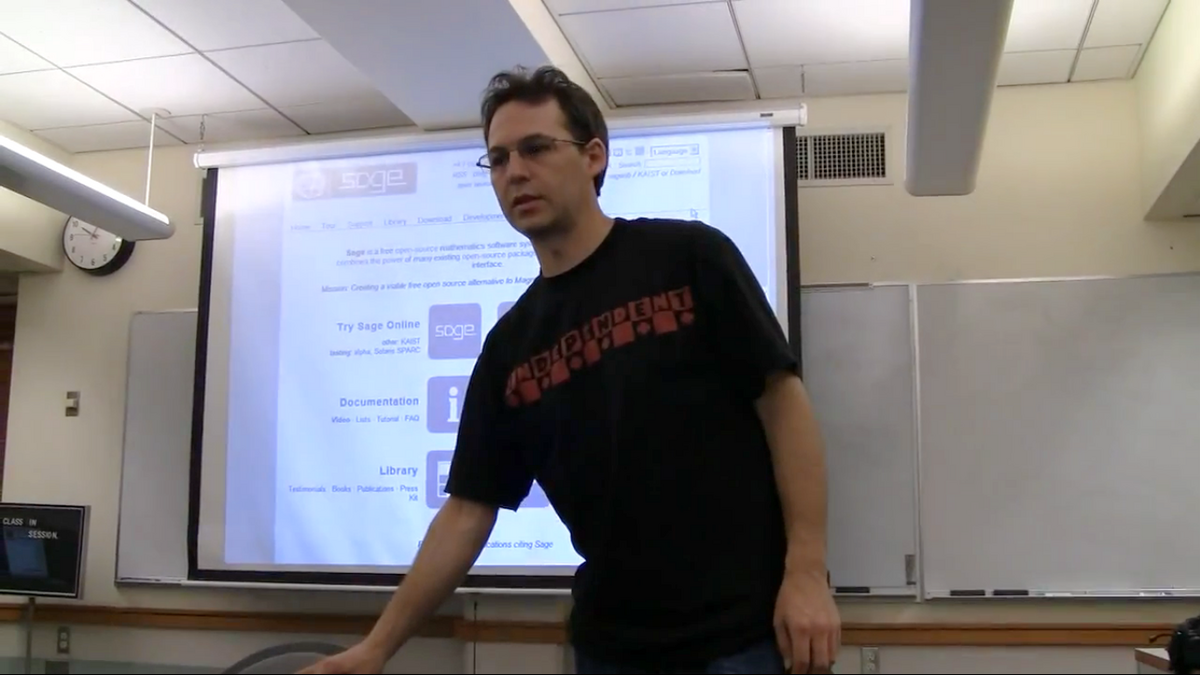
\includegraphics[width=0.7\linewidth]{images/screenshot006}
	\caption{William A. Stein đang nói chuyện về Sage tại REU Toán học năm 2011 tại Đại học Washington}
	\label{fig:screenshot006}
\end{figure}

William Stein, một nhà toán học chuyên về lý thuyết số, nhận thấy rằng các công cụ toán học mạnh mẽ hiện có đều yêu cầu chi phí cao và không thân thiện với người dùng trong cộng đồng nghiên cứu toán học. Với tư duy mã nguồn mở, ông đã quyết định xây dựng một nền tảng kết hợp từ nhiều công cụ toán học hiện có như:
\begin{itemize}
	\item \textbf{Maxima:} Hỗ trợ tính toán đại số trừu tượng.
	\item \textbf{NumPy và SciPy:} Tính toán số học và khoa học.
	\item \textbf{SymPy:} Tính toán trừu tượng.
	\item \textbf{R:} Phân tích thống kê.
	\item \textbf{Matplotlib:} Vẽ đồ thị và trực quan hóa.
\end{itemize}

\subsection{Quá trình phát triển}

Phiên bản đầu tiên của Sage được phát hành vào tháng 2 năm 2005 với tên gọi là "SAGE" (System for Algebra and Geometry Experimentation). Qua nhiều năm phát triển, Sage đã trở thành một hệ thống toán học hoàn chỉnh với khả năng tích hợp nhiều thư viện mạnh mẽ từ cộng đồng Python và các dự án mã nguồn mở khác.

Một cột mốc đáng chú ý trong lịch sử Sage là khi nó chuyển sang tên gọi chính thức là "SageMath" để nhấn mạnh vai trò là một hệ thống tính toán toán học. SageMath được sử dụng rộng rãi trong giảng dạy, nghiên cứu và công nghiệp nhờ tính linh hoạt và miễn phí của nó.

\subsection{Tính mã nguồn mở}

SageMath được phát triển dưới giấy phép GPL (GNU General Public License), nghĩa là bất kỳ ai cũng có thể sử dụng, sửa đổi và phân phối lại phần mềm. Điều này tạo ra một cộng đồng người dùng và phát triển lớn mạnh, với sự tham gia của nhiều nhà nghiên cứu và lập trình viên từ khắp nơi trên thế giới.

\subsection{Những cột mốc quan trọng}

\begin{itemize}
	\item \textbf{2005:} Phát hành phiên bản đầu tiên của SageMath.
	\item \textbf{2007:} SageMath giành giải thưởng FSF (Free Software Foundation) cho dự án phần mềm tự do.
	\item \textbf{2013:} Ra mắt CoCalc (trước đây là SageMathCloud), cho phép sử dụng SageMath trực tuyến.
	\item \textbf{2020:} SageMath được tích hợp hoàn chỉnh với Jupyter Notebook, tạo thuận lợi cho việc sử dụng trong môi trường tính toán khoa học.
\end{itemize}

\subsection{Tầm nhìn và tương lai}

Mục tiêu dài hạn của SageMath là trở thành một hệ thống tính toán toán học mạnh mẽ, thân thiện với người dùng và hoàn toàn miễn phí. SageMath đang tiếp tục được phát triển và hoàn thiện bởi cộng đồng mã nguồn mở, nhằm mở rộng hơn nữa khả năng tính toán và ứng dụng trong nhiều lĩnh vực khoa học, giáo dục và công nghiệp.

\section{So sánh SageMath với các phần mềm Toán học khác}
\begin{table}[H]
	\centering
	\begin{tabularx}{\textwidth}{|X|X|X|X|}
		\hline
		\textbf{Tiêu chí} & \textbf{SageMath} & \textbf{Mathematica / Maple} & \textbf{MATLAB} \\ \hline
		Mã nguồn & Mở hoàn toàn & Đóng & Đóng \\ \hline
		Ngôn ngữ lập trình & Python & Ngôn ngữ riêng biệt & MATLAB \\ \hline
		Tính toán trừu tượng (Symbolic) & Có (qua SymPy, Maxima) & Rất mạnh & Yếu \\ \hline
		Tính toán số & Mạnh (qua NumPy, SciPy) & Có & Rất mạnh \\ \hline
		Tính linh hoạt & Cao nhờ tích hợp nhiều thư viện & Trung bình & Trung bình \\ \hline
		Khả năng mở rộng & Dễ dàng thông qua thư viện Python & Hạn chế & Có nhưng không đa dạng như Python \\ \hline
		Chi phí sử dụng & Miễn phí & Trả phí cao & Trả phí cao \\ \hline
	\end{tabularx}
	\caption{So sánh SageMath với một số phần mềm toán học khác}
\end{table}

SageMath nổi bật nhờ khả năng tích hợp các thư viện hiện đại và tận dụng cộng đồng mã nguồn mở để phát triển liên tục.

\section{Hướng dẫn cài đặt SageMath}

\subsection*{Cài đặt trên Windows}

\begin{itemize}
	\item Truy cập trang chính thức: \texttt{https://www.sagemath.org/download.html}
	\item Tải bản cài đặt phù hợp với hệ điều hành.
	\item Cài đặt như một phần mềm thông thường.
	\item Đối với người dùng nâng cao, có thể sử dụng Windows Subsystem for Linux (WSL) để cài Sage trên Ubuntu.
\end{itemize}

\subsection*{Cài đặt trên Linux (Ubuntu)}

\begin{lstlisting}[language=bash]
	sudo apt update
	sudo apt install sagemath
\end{lstlisting}

\subsection*{Cài đặt trên macOS}

Có thể sử dụng Homebrew:

\begin{lstlisting}[language=bash]
	brew install --cask sagemath
\end{lstlisting}

\section{Sử dụng SageMath trực tuyến không cần cài đặt}

Trong trường hợp người dùng không muốn cài đặt SageMath trực tiếp trên máy tính, có thể sử dụng các nền tảng trực tuyến để chạy các mã SageMath mà không cần cấu hình phức tạp.

\subsection{CoCalc - Collaborative Calculation}

CoCalc (trước đây là SageMathCloud) là một dịch vụ trực tuyến giúp người dùng sử dụng SageMath ngay trên trình duyệt web mà không cần cài đặt. CoCalc hỗ trợ lập trình SageMath, Python, Jupyter Notebook và nhiều công cụ khác.
\begin{figure}[H]
	\centering
	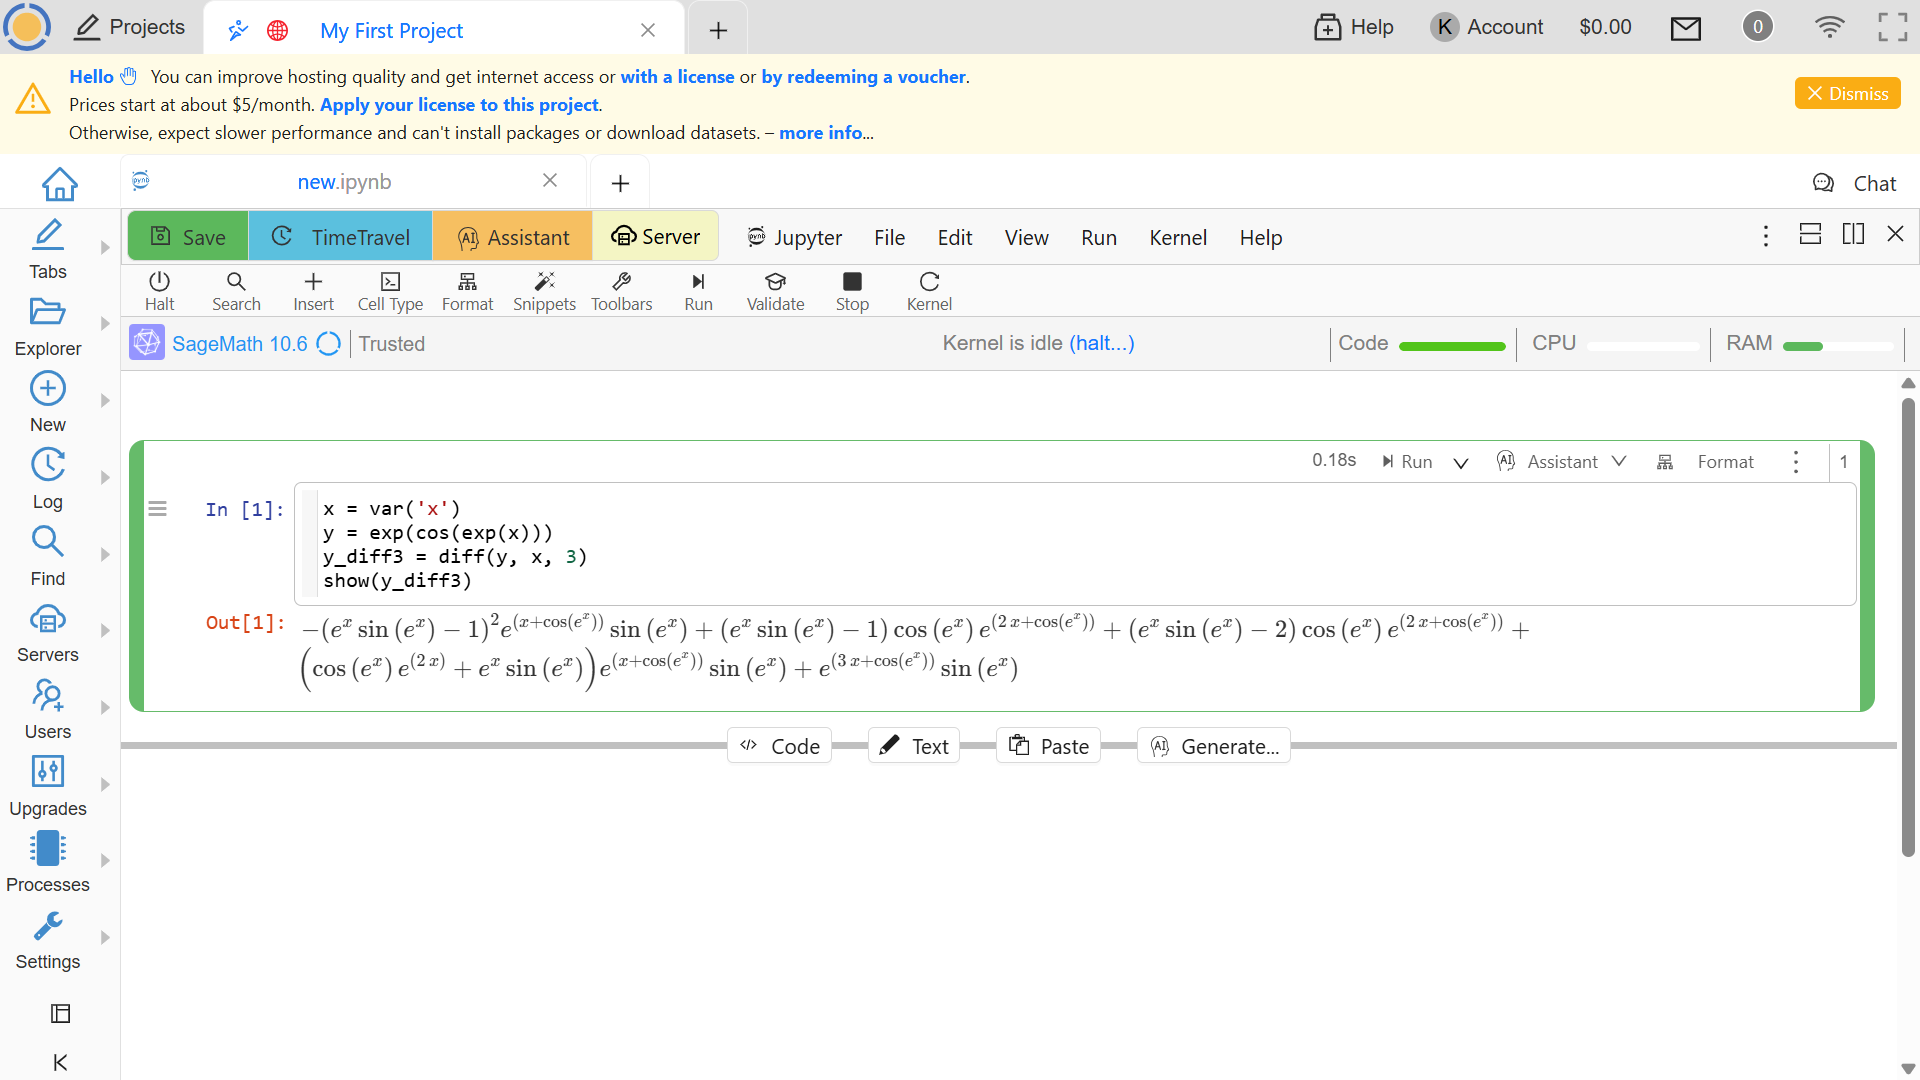
\includegraphics[width=0.7\linewidth]{images/screenshot004}
	\caption{Giao diện SageMath Notebook trên nền tảng trực tuyến CoCalc}
	\label{fig:screenshot004}
\end{figure}

\textbf{Hướng dẫn sử dụng CoCalc:}
\begin{itemize}
	\item Truy cập trang web: \url{https://cocalc.com}
	\item Đăng ký tài khoản hoặc sử dụng tài khoản Google để đăng nhập.
	\item Tạo một dự án mới (Project) và chọn môi trường SageMath.
	\item Tạo một file mới có phần mở rộng \texttt{.sagews} hoặc \texttt{.ipynb} để bắt đầu viết mã SageMath.
\end{itemize}

\textbf{Ưu điểm:}
\begin{itemize}
	\item Trực tiếp trên trình duyệt, không cần cài đặt.
	\item Hỗ trợ cộng tác và chia sẻ với người khác.
	\item Chạy được các notebook Jupyter có tích hợp SageMath.
\end{itemize}

\textbf{Nhược điểm:}
\begin{itemize}
	\item Phiên bản miễn phí có giới hạn tài nguyên.
	\item Cần kết nối internet ổn định.
\end{itemize}

\subsection{Binder - Chạy Notebook SageMath từ GitHub}

Binder là một dịch vụ trực tuyến cho phép chạy các notebook từ GitHub mà không cần cài đặt. Đây là giải pháp hiệu quả cho việc trình bày các đồ án và chia sẻ với giảng viên.
\begin{figure}[H]
	\centering
	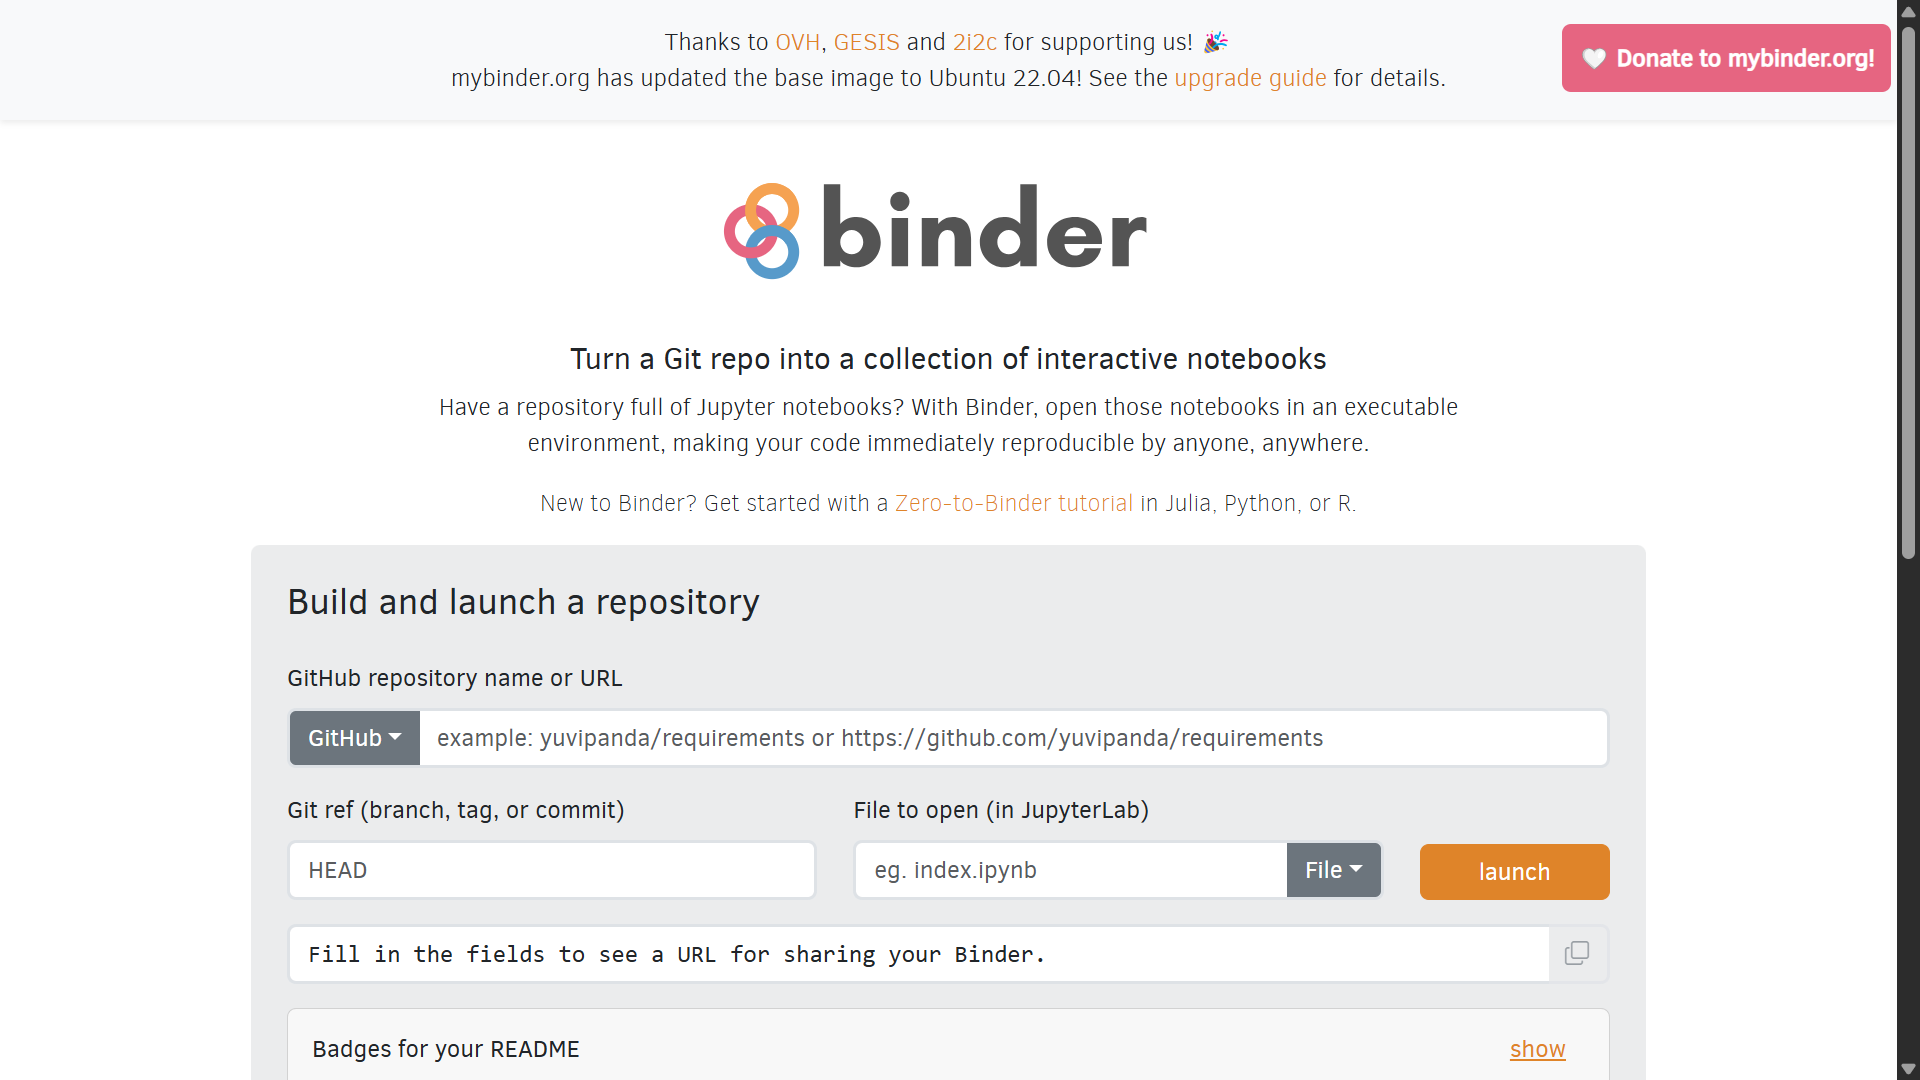
\includegraphics[width=0.7\linewidth]{images/screenshot003}
	\caption{Giao diện nền tảng Binder}
	\label{fig:screenshot003}
\end{figure}

\textbf{Hướng dẫn sử dụng Binder:}
\begin{itemize}
	\item Truy cập trang web: \url{https://mybinder.org}
	\item Nhập đường dẫn đến kho GitHub chứa file notebook.
	\item Chọn kernel SageMath nếu có, nhấn \texttt{Launch} để bắt đầu.
	\item Notebook sẽ được tải lên máy chủ và có thể chạy trực tuyến.
\end{itemize}

\textbf{Ưu điểm:}
\begin{itemize}
	\item Không cần đăng ký tài khoản.
	\item Dễ dàng chia sẻ với đường dẫn \textit{(link)} công khai.
\end{itemize}

\textbf{Nhược điểm:}
\begin{itemize}
	\item Khởi động lâu nếu dự án có nhiều thư viện.
	\item Không lưu lại trạng thái làm việc sau khi ngắt kết nối.
\end{itemize}

\subsection{Sage Cell - Tính toán nhanh với SageMath}

Sage Cell là công cụ trực tuyến cho phép thực thi các đoạn mã SageMath nhỏ mà không cần cài đặt.
\begin{figure}[H]
	\centering
	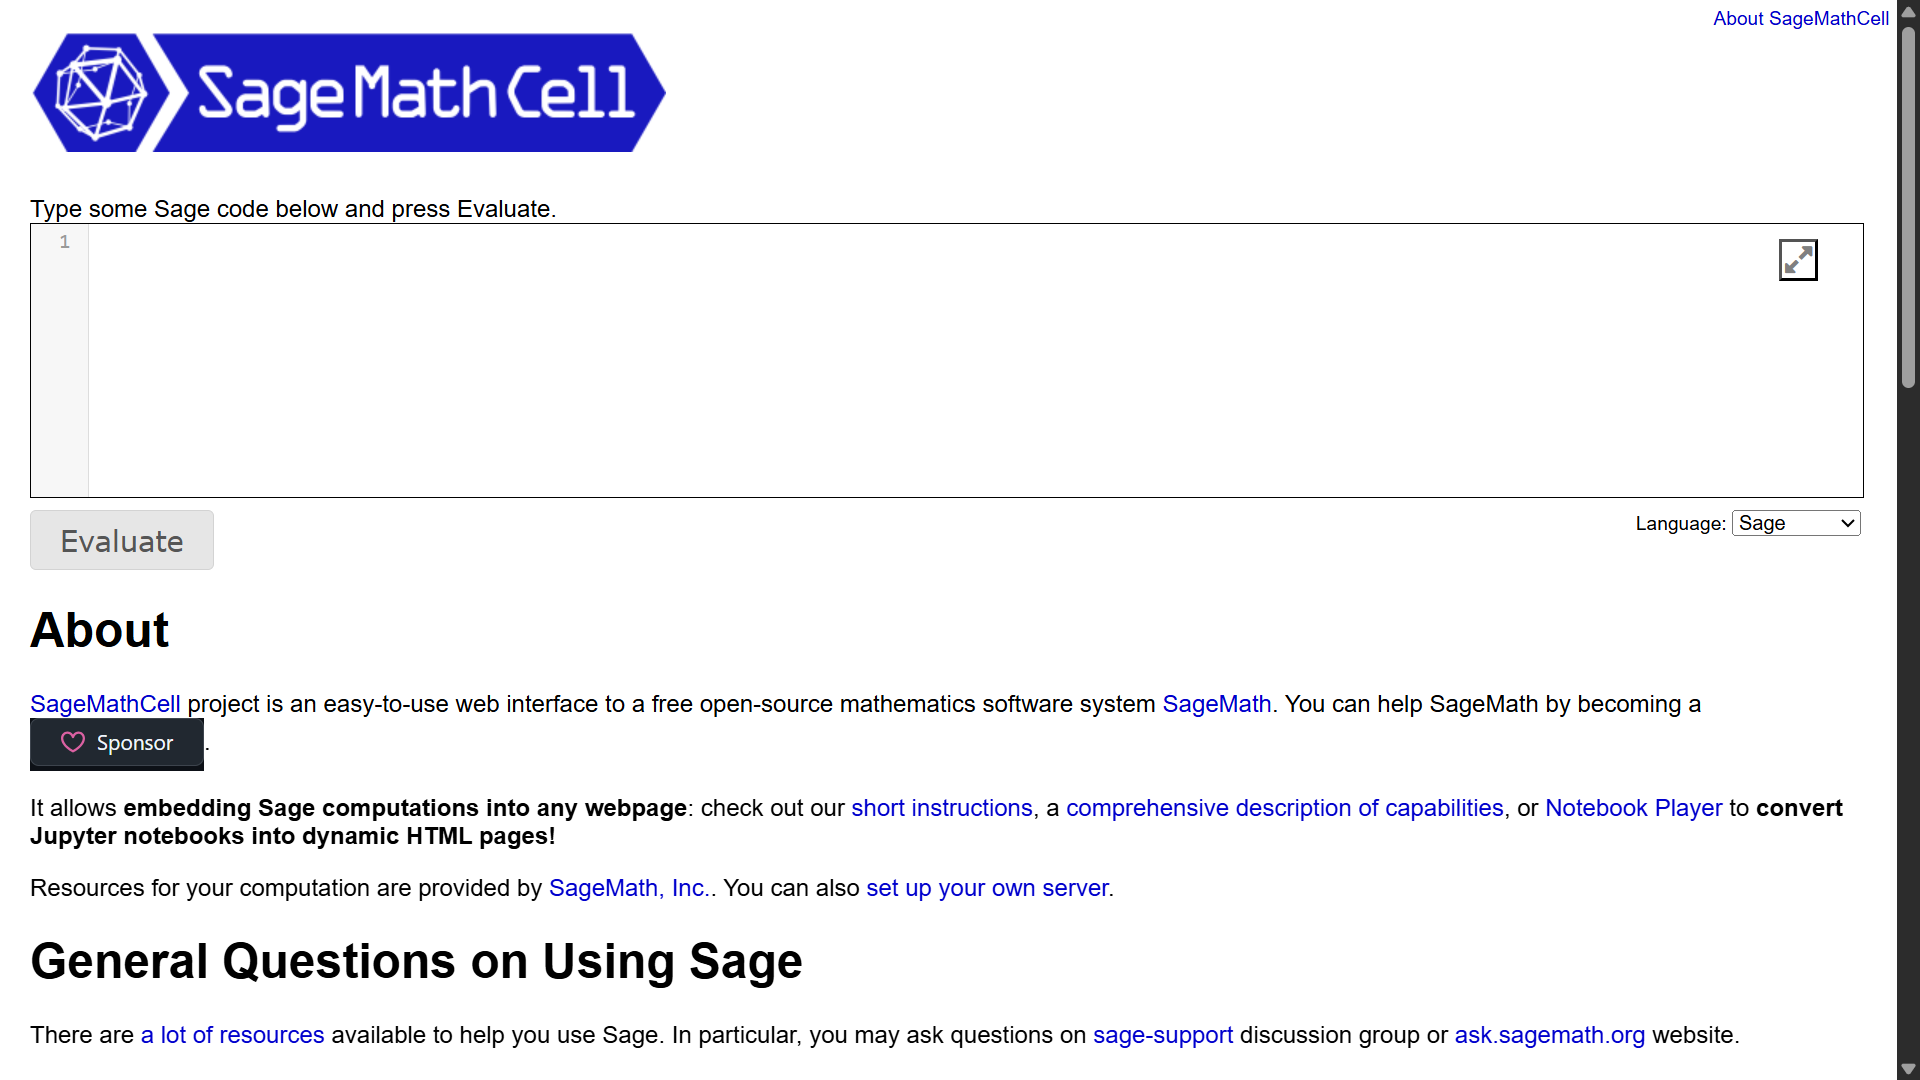
\includegraphics[width=0.7\linewidth]{images/screenshot002}
	\caption{Giao diện trang web Sage Cell}
	\label{fig:screenshot002}
\end{figure}

\textbf{Hướng dẫn sử dụng Sage Cell:}
\begin{itemize}
	\item Truy cập trang web: \url{https://sagecell.sagemath.org}
	\item Nhập mã SageMath vào ô nhập liệu.
	\item Nhấn \texttt{Evaluate} để xem kết quả.
\end{itemize}

\textbf{Ưu điểm:}
\begin{itemize}
	\item Nhanh chóng, không cần đăng nhập.
	\item Thích hợp cho các tính toán nhỏ.
\end{itemize}

\textbf{Nhược điểm:}
\begin{itemize}
	\item Không phù hợp với các dự án lớn hoặc tính toán phức tạp.
	\item Không có khả năng lưu trữ và cộng tác.
\end{itemize}

\subsection{So sánh các nền tảng trực tuyến}

\begin{table}[H]
	\centering
	\begin{tabular}{|c|c|c|c|}
		\hline
		\textbf{Nền tảng} & \textbf{Tính năng} & \textbf{Ưu điểm} & \textbf{Nhược điểm} \\
		\hline
		CoCalc & Tương tác mạnh mẽ & Hỗ trợ nhiều công cụ & Cần đăng ký tài khoản \\
		\hline
		Binder & Chạy từ GitHub & Dễ chia sẻ & Khởi động chậm \\
		\hline
		Sage Cell & Thực thi mã nhanh & Không cần đăng nhập & Chỉ tính toán nhỏ \\
		\hline
	\end{tabular}
	\caption{So sánh các nền tảng trực tuyến sử dụng SageMath}
\end{table}

\section{Giao diện và cách sử dụng cơ bản}

Sau khi cài đặt, người dùng có thể sử dụng SageMath theo các cách sau:

\begin{itemize}
	\item Giao diện dòng lệnh (CLI): khởi động bằng lệnh \texttt{sage}.
	\item Giao diện notebook (Jupyter): chạy lệnh \texttt{sage -n jupyter}.
	\item Giao diện đồ họa qua CoCalc nếu dùng trực tuyến.
\end{itemize}

\subsection*{Ví dụ cơ bản}

\begin{lstlisting}
	# Tinh tong 1 + 2 + ... + 100
	sum(i for i in (1..100))
	
	# Giai thua cua 10
	factorial(10)
	
	# Dao ham cua ham so
	f(x) = x^3 + x^2
	diff(f(x), x)
	
	# Ve do thi
	plot(sin(x), (x, -2*pi, 2*pi))
\end{lstlisting}

Sage hỗ trợ gần như toàn bộ các phép toán cơ bản đến nâng cao, cho phép nhập công thức trực tiếp theo cú pháp giống toán học thông thường.


	
	% Chương 3: Các tính năng cốt lõi của SageMath
	\chapter{Các tính năng cốt lõi của SageMath}
	\section{Ngôn ngữ và biểu thức cơ bản trong SageMath}
\subsection{Tổng quan cú pháp và quy tắc trong SageMath}

SageMath sử dụng cú pháp rất giống với Python, nhưng có một số điểm đặc biệt để hỗ trợ tính toán toán học. Dưới đây là một số quy tắc cơ bản mà người dùng cần nắm khi làm việc với SageMath.\\

\subsubsection{Quy tắc chung khi viết lệnh trong SageMath}
\begin{itemize}
	\item \textbf{Biến và tên hàm}: SageMath phân biệt chữ hoa và chữ thường, vì vậy \texttt{x} và \texttt{X} được coi là hai biến khác nhau. Cũng giống như Python, các biến và hàm có thể được sử dụng mà không cần khai báo kiểu dữ liệu.
	
	\item \textbf{Dấu cách}: Dấu cách không ảnh hưởng đến cú pháp trong SageMath, nhưng việc sử dụng dấu cách hợp lý sẽ giúp mã dễ đọc hơn và giảm khả năng xảy ra lỗi.
	
	\item \textbf{Ký tự toán học đặc biệt}: SageMath sử dụng các ký hiệu toán học quen thuộc như \texttt{+} (cộng), \texttt{-} (trừ), \texttt{*} (nhân), \texttt{/} (chia), cùng với nhiều toán tử khác để thực hiện các phép toán.
	
	\item \textbf{Lệnh kết thúc}: Không giống như nhiều ngôn ngữ lập trình khác, SageMath không yêu cầu dấu chấm phẩy (\texttt{;}) để kết thúc lệnh, tuy nhiên bạn vẫn có thể sử dụng dấu đó nếu muốn viết nhiều lệnh trên cùng một dòng.
\end{itemize}



\subsubsection{Cú pháp và quy tắc đặc biệt}

\begin{itemize}
	\item \textbf{Hàm số và đại số}: SageMath cung cấp nhiều hàm tích hợp sẵn để làm việc với biểu thức đại số, bao gồm các hàm lượng giác (\texttt{sin}, \texttt{cos}, \texttt{tan}), hàm mũ (\texttt{exp}), logarit (\texttt{log}), và nhiều hàm toán học khác.
	
	\item \textbf{Đặt tên cho biến}: Việc đặt tên cho biến trong SageMath cần tuân theo các quy tắc sau:
	\begin{itemize}
		\item Tên biến phải bắt đầu bằng một chữ cái (a–z, A–Z) hoặc dấu gạch dưới (\_).
		\item Các ký tự tiếp theo có thể là chữ cái, chữ số (0–9) hoặc dấu gạch dưới.
		\item Không được sử dụng các tên đã được định nghĩa trước trong SageMath, như các từ khóa hoặc tên hàm sẵn có (\texttt{sin}, \texttt{log}, \texttt{var}, \texttt{for}, \texttt{if}, \dots).
	\end{itemize}
\end{itemize}

\subsubsection{Chạy mã trong SageMath}
Để thực thi các lệnh trong SageMath, bạn có thể nhập trực tiếp vào terminal của SageMath hoặc sử dụng môi trường lập trình như Jupyter Notebook. Mã nguồn trong SageMath có thể được viết và lưu vào các file \texttt{.sage} hoặc \texttt{.py}.

Ví dụ về cách chạy một file \texttt{.sage}:

\begin{lstlisting}
	$ sage myscript.sage
\end{lstlisting}

Trong trường hợp bạn sử dụng Jupyter Notebook, bạn có thể chạy từng ô mã (\texttt{cell}) một cách độc lập.

\subsubsection{Quản lý và sử dụng thư viện trong SageMath}
SageMath cung cấp một hệ thống quản lý thư viện mạnh mẽ. Bạn có thể nhập thư viện vào mã của mình để mở rộng chức năng tính toán, ví dụ như nhập các thư viện đại số, giải tích, \dots

Ví dụ nhập thư viện để làm việc với các số nguyên lớn:

\begin{lstlisting}
	sage: from sage.modules.free_module import FreeModule
\end{lstlisting}


\subsection{Biến và kiểu dữ liệu cơ bản}

Trong SageMath, các biến và kiểu dữ liệu cơ bản được sử dụng để thực hiện các phép toán số học, đại số và nhiều phép toán khác. Việc hiểu rõ về các kiểu dữ liệu này là rất quan trọng khi làm việc với SageMath. Dưới đây là các kiểu dữ liệu cơ bản mà bạn sẽ gặp phải khi sử dụng SageMath.

\subsubsection{Khai báo và sử dụng biến}

Biến trong SageMath có thể được khai báo trực tiếp bằng cách gán giá trị cho chúng. SageMath hỗ trợ nhiều loại dữ liệu khác nhau, và bạn không cần phải chỉ định kiểu dữ liệu khi khai báo biến.

Ví dụ:

\begin{lstlisting}
	sage: x = 10  # Bien x la mot so nguyen
	sage: y = 3.14  # Bien y la mot so thuc
	sage: z = "SageMath"  # Bien z la mot chuoi
\end{lstlisting}

Ở trên, chúng ta đã khai báo ba biến với ba kiểu dữ liệu khác nhau:
\begin{itemize}
	\item \texttt{x} là số nguyên (\texttt{integer}),
	\item \texttt{y} là số thực (\texttt{float}),
	\item \texttt{z} là chuỗi ký tự (\texttt{string}).
\end{itemize}
\subsubsection{Kiểu dữ liệu cơ bản trong SageMath}

SageMath hỗ trợ một số kiểu dữ liệu cơ bản, bao gồm:

\begin{itemize}
	\item Số nguyên: Các số nguyên trong SageMath có thể có giá trị âm, dương hoặc bằng không.
	\item Số thực: Là các số có phần thập phân, được sử dụng để làm việc với các phép toán liên quan đến số học.
	\item Chuỗi: Là một chuỗi các ký tự, thường được sử dụng để lưu trữ văn bản.
	\item Danh sách: Là một kiểu dữ liệu để lưu trữ các giá trị trong một dãy. Các giá trị có thể là bất kỳ kiểu dữ liệu nào.
	\item Boolean: Kiểu dữ liệu Boolean có hai giá trị là \texttt{True} và \texttt{False}.
	\item Ma trận và vector: Được sử dụng để làm việc với đại số tuyến tính.
	\item Số nguyên lớn: SageMath hỗ trợ số nguyên có kích thước lớn hơn nhiều so với kiểu dữ liệu chuẩn của Python.
\end{itemize}

\subsubsection{Ví dụ về các kiểu dữ liệu trong SageMath}

Dưới đây là một số ví dụ về cách sử dụng các kiểu dữ liệu cơ bản trong SageMath.

\begin{lstlisting}
	sage: a = 15  # So nguyen
	sage: b = 3.5  # So thuc
	sage: c = "Hello, Sage!"  # Chuoi
	sage: lst = [1, 2, 3, 4, 5]  # Danh sach
	sage: flag = True  # Boolean
\end{lstlisting}

\subsubsection{Chuyển đổi giữa các kiểu dữ liệu}

SageMath cho phép bạn chuyển đổi giữa các kiểu dữ liệu khác nhau một cách dễ dàng.

Ví dụ, bạn có thể chuyển một số thực thành số nguyên:

\begin{lstlisting}
	sage: a = 5.7
	sage: int(a)  # Chuyen doi thanh so nguyen
	5
\end{lstlisting}

Hoặc chuyển đổi một chuỗi thành danh sách các ký tự:

\begin{lstlisting}
	sage: s = "Sage"
	sage: list(s)  # Chuyen doi thanh danh sach ki tu
	['S', 'a', 'g', 'e']
\end{lstlisting}

\subsubsection{Cách làm việc với các tập hợp}

SageMath cũng hỗ trợ kiểu dữ liệu tập hợp, cho phép bạn thực hiện các phép toán trên các tập hợp. Dưới đây là ví dụ về cách tạo và thao tác với tập hợp trong SageMath.

\begin{lstlisting}
	sage: A = Set([1, 2, 3, 4])
	sage: B = Set([3, 4, 5, 6])
	sage: A.union(B)  # Phep hop
	Set([1, 2, 3, 4, 5, 6])
	sage: A.intersubsection(B)  # Phep giao
	Set([3, 4])
\end{lstlisting}

\subsubsection{Thao tác với các số nguyên lớn}

Một trong những tính năng mạnh mẽ của SageMath là khả năng làm việc với các số nguyên lớn. Bạn có thể khai báo và thao tác với các số nguyên có giá trị cực kỳ lớn mà không gặp phải giới hạn như trong các ngôn ngữ lập trình khác.

Ví dụ:

\begin{lstlisting}
	sage: big_number = 123456789123456789123456789
	sage: big_number * 2  # Phep nhan voi mot so lon
	246913578246913578246913578
\end{lstlisting}

\subsection{Lệnh \texttt{show()} trong SageMath}

Lệnh \texttt{show()} trong SageMath dùng để hiển thị biểu thức, kết quả tính toán và trực quan hóa đồ thị dưới dạng ký hiệu toán học đẹp mắt.

\subsubsection{Hiển thị biểu thức toán học}

Lệnh \texttt{show()} giúp biểu diễn kết quả dưới dạng ký hiệu thay vì dạng văn bản thông thường.

\begin{lstlisting}
	# Hien thi bieu thuc
	sage: var('x')
	sage: f = x^2 + 2*x + 1
	sage: show(f)
\end{lstlisting}
	$$x^2 + 2x + 1$$

\subsubsection{Hiển thị đồ thị}

Lệnh \texttt{show()} được sử dụng để vẽ và hiển thị các đồ thị trong không gian 2D và 3D.

\begin{lstlisting}
	# Ve do thi ham so
	sage: plot(x^2, (x, -2, 2)).show()
\end{lstlisting}
\begin{figure}[H]
	\centering
	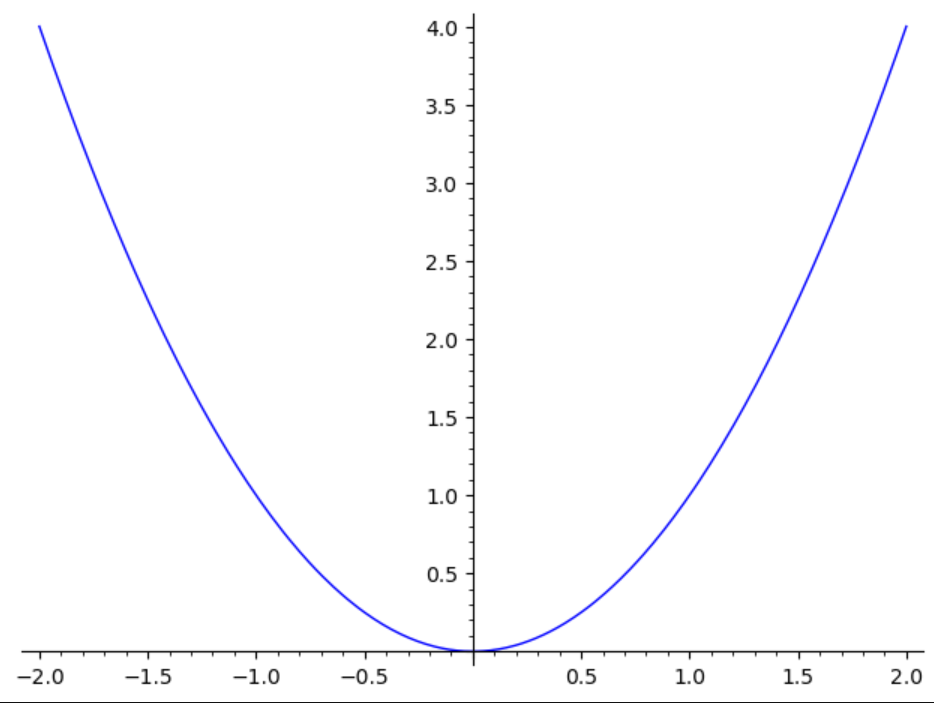
\includegraphics[width=0.7\linewidth]{images/screenshot007}
	\caption{Đồ thị hàm số $y=x^2$ trên đoạn $\left[-2,2\right]$}
	\label{fig:screenshot007}
\end{figure}

\subsubsection{Hiển thị ma trận}

\begin{lstlisting}
	# Hien thi ma tran
	sage: M = matrix([[1, 2], [3, 4]])
	sage: show(M)
\end{lstlisting}
$$\displaystyle \left(\begin{array}{rr}
	1 & 2 \\
	3 & 4
\end{array}\right)$$

Lệnh \texttt{show()} rất hữu ích khi cần trực quan hóa kết quả và trình bày các phép toán.

\subsection{Các phép toán số học và đại số cơ bản}

SageMath hỗ trợ một loạt các phép toán số học và đại số cơ bản, giúp người dùng thực hiện các phép toán cơ bản trong toán học như cộng, trừ, nhân, chia, và các phép toán đại số với các đối tượng phức tạp hơn như đa thức, số nguyên lớn, và các phép toán với các trường số học khác. Dưới đây là các phép toán cơ bản mà bạn sẽ sử dụng thường xuyên trong SageMath.

\subsubsection{Các phép toán số học cơ bản}

SageMath hỗ trợ các phép toán số học thông thường như cộng, trừ, nhân, chia, lũy thừa. Các phép toán này có thể được thực hiện trực tiếp trên các số nguyên, số thực hoặc các đối tượng số học khác.

Ví dụ về phép toán số học cơ bản:

\begin{lstlisting}
	sage: a = 10  # Phep gan
	sage: b = 5  # Phep gan
	sage: a + b  # Cong
	15
	sage: a - b  # Tru
	5
	sage: a * b  # Nhan
	50
	sage: a / b  # Chia
	2.0
	sage: a^b  # Luy thua
	100000
\end{lstlisting}

\subsubsection{Các phép toán với số nguyên lớn}

SageMath hỗ trợ làm việc với các số nguyên có độ dài lớn, vượt quá giới hạn của các kiểu dữ liệu số nguyên trong các ngôn ngữ lập trình khác. Điều này đặc biệt hữu ích khi làm việc với các bài toán lý thuyết số, mã hóa, và mật mã học.

Ví dụ:

\begin{lstlisting}
	sage: big_num = 123456789123456789123456789
	sage: big_num + 1000  # Phep cong voi so lon
	123456789123456789123457789
	sage: big_num * 1000000  # Phep nhan voi so lon
	123456789123456789123456789000000
\end{lstlisting}

\subsubsection{Các phép toán với đa thức}

SageMath hỗ trợ đầy đủ các phép toán đại số với đa thức, bao gồm cộng, trừ, nhân, chia, và các phép toán khác. Để làm việc với đa thức, bạn có thể sử dụng các hàm có sẵn trong SageMath như \texttt{PolynomialRing}.

Ví dụ về các phép toán với đa thức:

\begin{lstlisting}
	sage: R.<x> = PolynomialRing(QQ)  # Khai bao da thuc voi bien x
	sage: f = x^2 + 2*x + 1  # Da thuc f(x) = x^2 + 2x + 1
	sage: g = x^2 - 1  # Da thuc g(x) = x^2 - 1
	sage: f + g  # Cong hai da thuc
	x^2 + 2*x + 1 + x^2 - 1
	sage: f * g  # Nhan hai da thuc
	x^4 + 2*x^3 - x^2 - 2*x - 1
	sage: f / g  # Chia hai da thuc
	(x^2 + 2*x + 1)/(x^2 - 1)
\end{lstlisting}

\subsubsection{Phép chia lấy dư}

SageMath hỗ trợ phép chia lấy dư, cho phép bạn chia hai số nguyên và trả về thương và số dư. Điều này rất hữu ích trong lý thuyết số, đặc biệt là khi làm việc với các thuật toán như thuật toán Euclid.

Ví dụ về phép chia dư:

\begin{lstlisting}
	sage: a = 17
	sage: b = 5
	sage: divmod(a, b)  # Chia du giua 17 va 5
	(3, 2)  # (Thuong, So du)
\end{lstlisting}

\subsubsection{Các phép toán đại số cơ bản}

SageMath không chỉ hỗ trợ các phép toán số học cơ bản mà còn hỗ trợ các phép toán đại số với các đối tượng trừu tượng như nhóm, vành và trường.

Ví dụ về các phép toán nhóm:

\begin{lstlisting}
	sage: G = SymmetricGroup(3)  # Nhom doi xung S3
	sage: G[1] * G[2]  # Nhan hai phan tu trong nhom
	(1, 2)(3)
\end{lstlisting}

\subsubsection{Phép toán lũy thừa}

SageMath hỗ trợ các phép toán lũy thừa với các số nguyên, số thực và các đối tượng đại số. Phép toán lũy thừa có thể được thực hiện bằng ký hiệu mũ \texttt{\^} hoặc dùng hàm \texttt{pow()} (Hàm có sẵn trong ngôn ngữ Python).

Ví dụ về lũy thừa:

\begin{lstlisting}
	# Luy thua so nguyen
	sage: 2^5
	32
	
	# Cach khac su dung hai dau sao
	sage: 2**5
	32
	
	# Luy thua so thuc
	sage: 3.5^2
	12.25
	
	# Cach khac voi so thuc
	sage: pow(3.5, 2)
	12.25
\end{lstlisting}

\textbf{Lưu ý:} Ký hiệu \texttt{**} tương tự như \texttt{\^} để tính lũy thừa, nhưng trong một số trường hợp, \texttt{**} được ưu tiên hơn để tránh lỗi cú pháp.


\section{Đại số, giải tích và hình học}
\subsection{Làm việc với phương trình và hệ phương trình}

Trong SageMath, bạn có thể giải các phương trình đại số đơn giản đến phức tạp, bao gồm phương trình bậc một, bậc hai, và hệ phương trình đại số. SageMath cung cấp các công cụ mạnh mẽ để giải phương trình với một biến hoặc nhiều biến, đồng thời hỗ trợ các phương trình với các hệ số phức tạp.

\subsubsection{Giải phương trình đơn biến}

Để giải một phương trìnhn, bạn có thể sử dụng hàm \texttt{solve()}, nơi đầu vào là phương trình cần giải.

Ví dụ về giải phương trình bậc nhất một ẩn:

\begin{lstlisting}
	sage: x = var('x')  # Dinh nghia bien x
	sage: solve(x + 5 == 0, x)  # Giai phuong trinh x + 5 = 0
	[x == -5]
\end{lstlisting}

SageMath trả về kết quả dưới dạng danh sách các nghiệm. Trong ví dụ trên, phương trình \(x + 5 = 0\) có nghiệm \(x = -5\).

Ví dụ về giải phương trình bậc hai:

\begin{lstlisting}
	sage: solve(x^2 + 5*x + 6 == 0, x)  # Giai phuong trinh bac hai x^2 + 5x + 6 = 0
	[x == -3, x == -2]
\end{lstlisting}

Phương trình bậc hai \(x^2 + 5x + 6 = 0\) có hai nghiệm là \(x = -2\) và \(x = -3\).

\subsubsection{Giải phương trình đa biến}

SageMath cũng hỗ trợ giải các phương trình có nhiều biến. Bạn có thể định nghĩa nhiều biến và sử dụng hàm \texttt{solve()} để giải các hệ phương trình.

Ví dụ về giải hệ phương trình với hai biến:

\begin{lstlisting}
	sage: y = var('y')  # Dinh nghia them bien y
	sage: solve([x + y == 3, x - y == 1], x, y)  # Giai he phuong trinh x + y = 3 va x - y = 1
	[x == 2, y == 1]
\end{lstlisting}

Kết quả là hệ phương trình có nghiệm \(x = 2\) và \(y = 1\).

\subsubsection{Giải phương trình với các hệ số phức tạp}

SageMath cũng cho phép bạn giải các phương trình với các hệ số phức tạp, bao gồm số phức hoặc các biểu thức đại số phức tạp.

Ví dụ về giải phương trình với số phức:

\begin{lstlisting}
	sage: z = var('z', domain=CC)  # Dinh nghia bien Z trong tap so phuc
	sage: solve(z^2 + 1 == 0, z)  # Giai phuong trinh z^2 + 1 = 0 trong tap so phuc
	[z == -I, z == I]
\end{lstlisting}

Phương trình \(z^2 + 1 = 0\) có hai nghiệm là \(z = i\) và \(z = -i\), với \(i\) là đơn vị ảo.

\subsubsection{Giải hệ phương trình đại số phi tuyến}

SageMath cũng hỗ trợ giải các hệ phương trình đại số phi tuyến, bao gồm các phương trình bậc cao hoặc các phương trình có hàm số phi tuyến.

Ví dụ về hệ phương trình phi tuyến:

\begin{lstlisting}
	sage: solve([x^2 + y^2 == 1, x^2 - y^2 == 0], x, y)  # Giai he phuong trinh phi tuyen
	[x == sqrt(2)/2, y == sqrt(2)/2]
\end{lstlisting}

Hệ phương trình đại số phi tuyến \(x^2 + y^2 = 1\) và \(x^2 - y = 0\) có nghiệm \(x = \frac{\sqrt{2}}{2}\) và \(y = \frac{\sqrt{2}}{2}\).

\subsubsection{Sử dụng phương trình trong các bài toán ứng dụng}

SageMath không chỉ giải các phương trình đơn giản mà còn được sử dụng để giải các phương trình trong các bài toán ứng dụng. Bạn có thể sử dụng phương trình để mô hình hóa các bài toán trong các lĩnh vực như vật lý, kỹ thuật, kinh tế học, và khoa học máy tính.

Ví dụ về bài toán mô phỏng sự rơi tự do của vật thể:

\begin{lstlisting}
	sage: t = var('t')  # Dinh nghia bien thoi gian t
	sage: h = 100 - 5*t^2  # Phuong trinh mo ta chieu cao cua vat the theo thoi gian t
	solve(h == 0, t)  # Tim thoi gian vat the cham dat (khi h = 0)
	[t == -2*sqrt(5), t == 2*sqrt(5)]
\end{lstlisting}

Kết quả là \(t = \sqrt{20}\), nghĩa là vật thể chạm đất sau khoảng 4.47 giây.


\subsection{Tính toán đại số trừu tượng (nhóm, vành, trường, đa thức)}

SageMath cung cấp các công cụ mạnh mẽ để làm việc với đại số trừu tượng, bao gồm các cấu trúc đại số cơ bản như vành, nhóm, trường và các phép toán với đa thức. Các cấu trúc này đóng vai trò quan trọng trong các bài toán toán học, vật lý và khoa học máy tính.

\subsubsection{Làm việc với nhóm}

Nhóm là một tập hợp các phần tử với một phép toán nhị phân thỏa mãn các tính chất: đóng, có phần tử trung tính, mỗi phần tử có phần tử nghịch đảo.

Ví dụ về nhóm phép cộng trên các số nguyên modulo 7:

\begin{lstlisting}
	sage: G = Group([1, 2, 3, 4, 5, 6], operation='addition mod 7')  # Nhom cac so nguyen modulo voi phep cong
	sage: G.is_group()  # Kiem tra G co la 1 nhom khong
	True
\end{lstlisting}

Phép toán `operation='addition mod 7'` xác định phép cộng trong nhóm modulo 7. SageMath cung cấp phương thức \texttt{is\_group()} để kiểm tra xem tập hợp có là một nhóm không.

\subsubsection{Làm việc với vành}

Vành là một cấu trúc đại số có hai phép toán: cộng và nhân, và phải thỏa mãn một số tính chất nhất định. Ví dụ về vành các số nguyên modulo 7:

\begin{lstlisting}
	sage: R = Ring([0, 1, 2, 3, 4, 5, 6], addition='mod 7', multiplication='mod 7')  # Vanh cac so nguyen modulo 7
	sage: R.is_ring()  # Kiem tra R co la 1 vanh khong
	True
\end{lstlisting}

Trong ví dụ này, ta tạo ra một vành với phép cộng và phép nhân là phép toán modulo 7.

\subsubsection{Làm việc với trường}

Trường là một cấu trúc đại số trong đó các phép toán cộng, trừ, nhân và chia đều được xác định và có tính nghịch đảo. Trường phổ biến nhất là trường số thực và số phức.

Ví dụ về trường số thực:

\begin{lstlisting}
	sage: F = RealField()  # Tao truong so thuc
	sage: F.is_field()  # Kiem tra F co la 1 truong khong
	True
\end{lstlisting}

SageMath cũng hỗ trợ các trường hữu hạn. Ví dụ về trường hữu hạn:

\begin{lstlisting}
	sage: GF(7)  # Truong huu han F_7
	GF(7)
\end{lstlisting}

Trường này bao gồm các phần tử \{0, 1, 2, 3, 4, 5, 6\}, và các phép toán cộng, nhân, chia đều được thực hiện modulo 7.

\subsubsection{Làm việc với đa thức}

SageMath cung cấp các công cụ mạnh mẽ để làm việc với đa thức, từ các phép toán cơ bản đến các phép toán phức tạp. Bạn có thể thực hiện cộng, trừ, nhân, chia đa thức, giải phương trình đa thức, và làm việc với các đa thức trong các trường hoặc vành.

Ví dụ về tạo đa thức trong một biến:

\begin{lstlisting}
	sage: R.<x> = PolynomialRing(ZZ)  # Tao da thuc trong vanh da thuc co he so nguyen
	sage: p = x^2 + 2*x + 1  # Dinh nghia da thuc
	sage: p.factor()  # Phan tich da thuc thanh nhan tu
	(x + 1)^2
\end{lstlisting}

SageMath phân tích đa thức \(x^2 + 2x + 1\) thành \((x + 1)^2\), điều này giúp ích trong việc giải các phương trình đa thức.

Ví dụ về chia đa thức:

\begin{lstlisting}
	sage: q, r = (x^3 + 2*x^2 + x + 1).div(x^2 + x)  # Chia da thuc
	sage: q, r  # Thuong va phan du
	(x + 1, 1)
\end{lstlisting}

Ở đây, \(x^3 + 2x^2 + x + 1\) chia cho \(x^2 + x\) có thương là \(x + 1\) và phần dư là 1.

\subsubsection{Làm việc với vành đa thức}

Trong SageMath, bạn có thể làm việc với các vành đa thức, nơi phép cộng và nhân được xác định trên các đa thức.

Ví dụ về vành đa thức:

\begin{lstlisting}
	sage: R.<x> = PolynomialRing(ZZ, 'x')  # Vanh cac da thuc voi he so la so nguyen
	sage: I = ideal(x^2 + 1, R)  # Dinh nghia mien cua vanh da thuc
	sage: I.is_ideal()  # Kiem tra I co la mot ideal khong
	True
\end{lstlisting}


\subsection{Ma trận, vector và đại số tuyến tính}

SageMath cung cấp các công cụ mạnh mẽ để làm việc với ma trận, vector và thực hiện các phép toán đại số tuyến tính. Các phép toán này rất quan trọng trong các lĩnh vực như học máy, kỹ thuật, khoa học dữ liệu, và các nghiên cứu toán học.

\subsubsection{Làm việc với vector}

Vector là các đối tượng có thể đại diện cho các điểm trong không gian hoặc các phép toán đại số tuyến tính. Trong SageMath, vector có thể được định nghĩa trong các không gian số học khác nhau như \(\mathbb{R}^n\) hoặc \(\mathbb{C}^n\).

Ví dụ tạo một vector trong không gian thực:

\begin{lstlisting}
	sage: v = vector([1, 2, 3])  # Vector trong khong gian R^3
	sage: v
	(1, 2, 3)
\end{lstlisting}

Bạn có thể thực hiện các phép toán cơ bản trên vector như cộng, trừ, nhân với một số vô hướng (scalar), và tính độ dài:

\begin{lstlisting}
	sage: v + vector([4, 5, 6])  # Cong vector
	(5, 7, 9)
	sage: v * 2  # Nhan vector voi mot so vo huong
	(2, 4, 6)
	sage: v.norm()  # Tinh do dai cua vector
	3.7416573867739413
\end{lstlisting}

Ngoài các phép toán cơ bản, bạn cũng có thể tính tích vô hướng và tích có hướng của các vector. 

Tích vô hướng của hai vector là một phép toán trả về một số vô hướng, được tính bằng tổng các tích của các thành phần tương ứng của hai vector. Ví dụ:

\begin{lstlisting}
	sage: u = vector([1, 2, 3])
	sage: w = vector([4, 5, 6])
	sage: u.dot_product(w)  # Tich vo huong
	32
\end{lstlisting}

Tích có hướng (hoặc tích chéo) là một phép toán giữa hai vector trong không gian ba chiều, cho ra một vector vuông góc với cả hai vector ban đầu. Ví dụ:

\begin{lstlisting}
	sage: u.cross_product(w)  # Tich co huong
	(-3, 6, -3)
\end{lstlisting}


\subsubsection{Làm việc với ma trận}

Ma trận là các bảng số học dùng để biểu diễn các hệ phương trình tuyến tính, phép biến đổi tuyến tính, hoặc các phép toán đại số tuyến tính khác. SageMath cho phép bạn dễ dàng tạo ma trận và thực hiện các phép toán trên ma trận như cộng, nhân, tính định thức, và nghịch đảo.

Ví dụ tạo một ma trận và thực hiện phép cộng:

\begin{lstlisting}
	sage: M = Matrix([[1, 2], [3, 4]])  # Ma tran 2x2
	sage: M
	[1 2]
	[3 4]
	sage: M + Matrix([[5, 6], [7, 8]])  # Cong hai ma tran
	[6 8]
	[10 12]
\end{lstlisting}

Phép nhân ma trận:

\begin{lstlisting}
	sage: M * Matrix([[5], [6]])  # Nhan ma tran voi vector
	[17]
	[39]
\end{lstlisting}

Tính định thức của ma trận:

\begin{lstlisting}
	sage: M.det()  # Tinh dinh thuc cua ma tran
	-2
\end{lstlisting}

Tính nghịch đảo của ma trận (nếu có):

\begin{lstlisting}
	sage: M.inv()  # Tinh ma tran nghich dao
	[-2.0  1.0]
	[ 1.5 -0.5]
\end{lstlisting}

\subsubsection{Làm việc với hệ phương trình tuyến tính}

SageMath hỗ trợ giải các hệ phương trình tuyến tính bằng cách sử dụng ma trận. Ví dụ, để giải một hệ phương trình tuyến tính \(A \cdot x = b\), bạn có thể sử dụng phương thức \texttt{solve()}.

Giải hệ phương trình \( \begin{bmatrix} 1 & 2 \\ 3 & 4 \end{bmatrix} \cdot \begin{bmatrix} x_1 \\ x_2 \end{bmatrix} = \begin{bmatrix} 5 \\ 6 \end{bmatrix} \):

\begin{lstlisting}
	sage: A = Matrix([[1, 2], [3, 4]])  # Ma tran he phuong trinh
	sage: b = vector([5, 6])  # Vector ben phai
	sage: A.solve_right(b)  # Giai he phuong trinh
	(0, 1)
\end{lstlisting}

Phương thức \texttt{solve\_right()} trả về nghiệm của hệ phương trình.

\subsubsection{Giá trị riêng và vectơ riêng}

Một trong những phép toán quan trọng trong đại số tuyến tính là tính giá trị riêng và vectơ riêng của ma trận. SageMath cung cấp phương thức \texttt{eigenvalues()} và \texttt{eigenvectors()} để tính toán các giá trị này.

Tính giá trị riêng của ma trận:

\begin{lstlisting}
	sage: M.eigenvalues()  # Tinh gia tri rieng cua ma tran
	[5.0, -0.9999999999999999]
\end{lstlisting}

Tính vectơ riêng của ma trận:

\begin{lstlisting}
	sage: M.eigenvectors()  # Tinh vector rieng cua ma tran
	[(5.0, 1, [(1, 1)]), (-1.0, 1, [(1, -2)])]
\end{lstlisting}

\subsubsection{Các phép toán đại số tuyến tính khác}

SageMath hỗ trợ nhiều phép toán đại số tuyến tính khác như phân rã ma trận, giải các hệ phương trình, và tính toán với không gian vector. Các phương thức khác bao gồm:

- \texttt{row\_space()}, \texttt{column\_space()}: Tính không gian hàng và không gian cột.
- \texttt{rank()}: Tính hạng của ma trận.
- \texttt{eigenvalues()}: Tính giá trị riêng.
- \texttt{svd()}: Phân rã giá trị kỳ dị (Singular Value Decomposition).

Ví dụ tính hạng ma trận:

\begin{lstlisting}
	sage: M.rank()  # Tinh hang cua ma tran
	2
\end{lstlisting}

\subsection{Đạo hàm, tích phân và giải tích}

SageMath hỗ trợ tính toán đạo hàm, tích phân và các phép toán giải tích khác như giải phương trình vi phân, tính toán số học chính xác cao, và làm việc với các hàm số. Phần này sẽ trình bày cách sử dụng các công cụ giải tích cơ bản trong SageMath để giải quyết các bài toán toán học liên quan đến đạo hàm, tích phân và các phép toán tiếp theo.

\subsubsection{Đạo hàm}

Đạo hàm là một trong những phép toán cơ bản trong giải tích. SageMath cung cấp chức năng để tính đạo hàm của các hàm số, bao gồm cả đạo hàm riêng và đạo hàm toàn phần.

Ví dụ tính đạo hàm của hàm số \(f(x) = x^2 + 3x + 5\):

\begin{lstlisting}
	sage: x = var('x')  # Dinh nghia bien x
	sage: f = x^2 + 3*x + 5  # Dinh nghia ham so
	sage: diff(f, x)  # Tinh dao ham cua f theo x
	2*x + 3
\end{lstlisting}

SageMath cũng cho phép tính đạo hàm bậc cao:

\begin{lstlisting}
	sage: diff(f, x, 2)  # Dao ham bac 2 cua f
	2
\end{lstlisting}

\subsubsection{Tích phân}

Tích phân là phép toán cơ bản trong giải tích, được sử dụng để tính diện tích dưới đường cong, thể tích và nhiều ứng dụng khác. SageMath hỗ trợ tính tích phân bất định và tích phân xác định.

Tính tích phân bất định của hàm \(f(x) = x^2 + 3x + 5\):

\begin{lstlisting}
	sage: integrate(f, x)  # Tinh tich phan bat dinh cua f theo x
	x^3/3 + 3*x^2/2 + 5*x
\end{lstlisting}

Tính tích phân xác định của hàm \(f(x) = x^2\) từ \(x = 0\) đến \(x = 1\):

\begin{lstlisting}
	sage: integrate(x^2, (x, 0, 1))  # Tinh tich phan xac dinh cua x^2 tu 0 den 1
	1/3
\end{lstlisting}

\subsubsection{Giải phương trình vi phân}

SageMath cũng hỗ trợ giải phương trình vi phân (ODEs), bao gồm các phương trình vi phân thường và các phương trình vi phân riêng. Dưới đây là ví dụ về cách giải một phương trình vi phân thông qua phương thức \texttt{desolve()}.

Giải phương trình vi phân \(y' = -2y\) với điều kiện ban đầu \(y(0) = 1\):

\begin{lstlisting}
	sage: y = function('y')(x)  # Dinh nghia ham y(x)
	sage: desolve(-2*y, y, ics=[0,1])  # Giai phuong trinh vi phan voi dieu kien ban dau
	exp(-2*x)
\end{lstlisting}

\subsubsection{Tính toán với chuỗi số học}

SageMath cũng có thể tính toán với chuỗi số học (series), bao gồm các chuỗi hội tụ và phân kỳ. Ví dụ tính chuỗi Taylor của hàm \(\sin(x)\) tại \(x = 0\).

\begin{lstlisting}
	sage: taylor(sin(x), x, 0, 5)  # Tinh chuoi Taylor bac 5 cua sin(x) tai x=0
	x - x^3/6 + O(x^5)
\end{lstlisting}

\subsection{Chuỗi, giới hạn và phép tính xấp xỉ}

SageMath cung cấp các công cụ mạnh mẽ để làm việc với chuỗi số học, tính toán giới hạn và thực hiện các phép tính xấp xỉ. Những công cụ này rất hữu ích khi làm việc với các chuỗi hội tụ hoặc phân kỳ, tính toán giới hạn của các hàm số tại một điểm, và áp dụng các phương pháp xấp xỉ trong các bài toán toán học phức tạp.

\subsubsection{Chuỗi số học}

Chuỗi số học trong SageMath được sử dụng để tính toán và phân tích các chuỗi vô hạn. Các chuỗi này có thể hội tụ hoặc phân kỳ, và việc tính toán các giới hạn của chúng là rất quan trọng trong giải tích.

Ví dụ tính chuỗi của hàm số \(f(x) = \frac{1}{n^2}\) từ \(n = 1\) đến \(n = \infty\):

\begin{lstlisting}
	sage: summation(1/n^2, n, 1, infinity)  # Tinh tong cua chuoi 1/n^2 tu n=1 den vo cung
	pi^2/6
\end{lstlisting}

SageMath có thể tính chuỗi vô hạn và xác định tổng của chuỗi hội tụ như trong ví dụ trên.

\subsubsection{Giới hạn của hàm số}

Giới hạn là một trong những công cụ cơ bản trong giải tích, giúp xác định hành vi của một hàm số khi biến số tiến gần đến một giá trị nhất định. SageMath hỗ trợ tính giới hạn của các hàm số tại một điểm.

Ví dụ tính giới hạn của hàm số \(f(x) = \frac{1}{x}\) khi \(x\) tiến đến \(0\):

\begin{lstlisting}
	# Tinh gioi han cua 1/x khi x tien den 0 tu ben phai
	sage: limit(1/x, x=0, dir='plus')
	+Infinity
	
	# Tinh gioi han cua 1/x khi x tien den 0 tu ben trai
	sage: limit(1/x, x=0, dir='minus')
	-Infinity
\end{lstlisting}

SageMath tự động tính toán giới hạn của các hàm số tại các điểm mà hàm có thể hội tụ hoặc phân kỳ.

\subsubsection{Phép tính xấp xỉ}

SageMath cung cấp nhiều phương pháp để tính xấp xỉ các giá trị của các hàm số, đặc biệt hữu ích khi làm việc với các giá trị không thể tính chính xác hoặc khi cần tốc độ tính toán nhanh.

Ví dụ, tính giá trị xấp xỉ của hàm \(\sin(x)\) tại \(x = 1\) với 10 chữ số thập phân:

\begin{lstlisting}
	sage: sin(1).n(digits=10)  # Tinh gia tri xap xi cua sin(1) voi 10 chu so thap phan
	0.8414710000
\end{lstlisting}

SageMath hỗ trợ tính xấp xỉ cho các phép toán phức tạp, giúp tiết kiệm thời gian tính toán khi không cần độ chính xác tuyệt đối.

\subsubsection{Chuyển đổi giữa chuỗi và số thực}

SageMath cho phép chuyển đổi giữa chuỗi số học và các số thực. Điều này rất hữu ích khi làm việc với các chuỗi số học mà bạn muốn tính toán các giá trị thực gần đúng.

Ví dụ, chuyển đổi chuỗi \( \sum_{n=1}^{\infty} \frac{1}{n^2} \) thành giá trị thực:

\begin{lstlisting}
	sage: summation(1/n^2, n, 1, infinity).n()  # Tinh gia tri gan dung cua chuoi
	1.6449340668
\end{lstlisting}

SageMath cho phép bạn dễ dàng chuyển đổi giữa các biểu thức chính xác và các giá trị số học gần đúng, giúp tiện lợi trong tính toán.


\subsection{Làm việc với hàm số và biểu đồ (vẽ đồ thị 2D, 3D)}

SageMath cung cấp các công cụ mạnh mẽ để làm việc với hàm số và vẽ đồ thị, giúp trực quan hóa các kết quả toán học một cách dễ dàng và hiệu quả. Các đồ thị 2D và 3D có thể được tạo ra cho các hàm số, cung cấp cái nhìn sâu sắc về đặc tính và hành vi của hàm.

\subsubsection{Vẽ đồ thị 2D của hàm số}

Để vẽ đồ thị 2D trong SageMath, bạn có thể sử dụng hàm \texttt{plot}, cho phép vẽ đồ thị của một hàm số trên một khoảng xác định. 

Ví dụ vẽ đồ thị của hàm \( f(x) = \sin(x) \) trên đoạn \( [0, 2\pi] \):

\begin{lstlisting}
	sage: plot(sin(x), (x, 0, 2*pi))  # Ve do thi cua sin(x) tu 0 den 2*pi
\end{lstlisting}
\begin{figure}
	\centering
	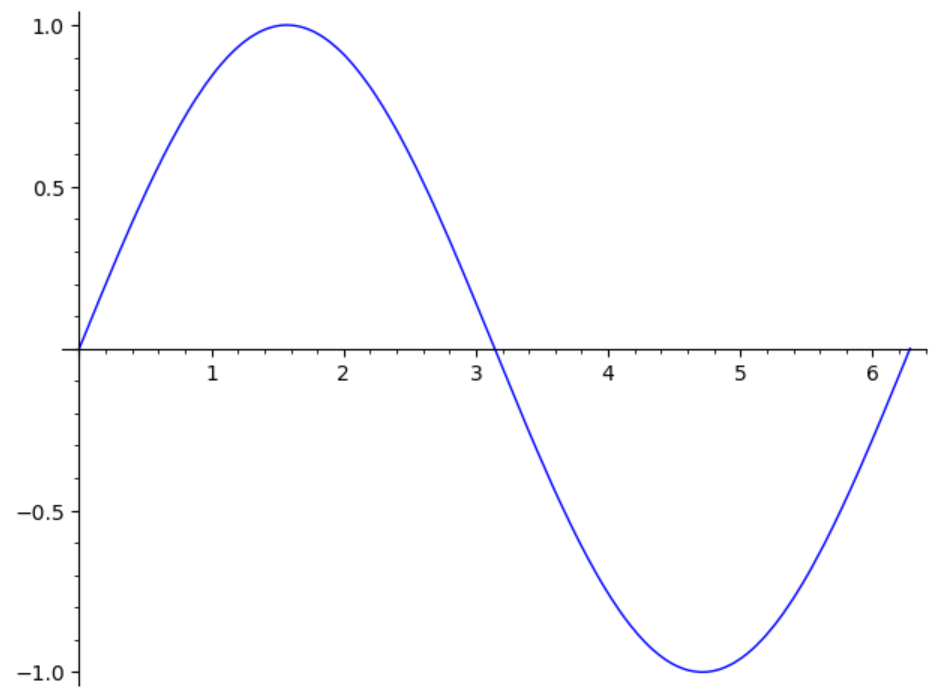
\includegraphics[width=0.7\linewidth]{images/screenshot008}
	\caption{Đồ thị 2D của hàm số \(\sin(x)\) trên đoạn \( [0, 2\pi] \)}
	\label{fig:screenshot008}
\end{figure}

\subsubsection{Vẽ đồ thị 2D của nhiều hàm số}

SageMath hỗ trợ vẽ đồ thị của nhiều hàm số trên cùng một đồ thị. Bạn có thể vẽ nhiều hàm số trên cùng một biểu đồ bằng cách sử dụng toán tử cộng (\(+\)).

Ví dụ, vẽ đồ thị của \( f(x) = \sin(x) \) và \( g(x) = \cos(x) \) trên cùng một đồ thị:

\begin{lstlisting}
	sage: plot(sin(x), (x, 0, 2*pi)) + plot(cos(x), (x, 0, 2*pi))  # Ve dong thoi do thi cua ham sin(x) va cos(x)
\end{lstlisting}
\begin{figure}
	\centering
	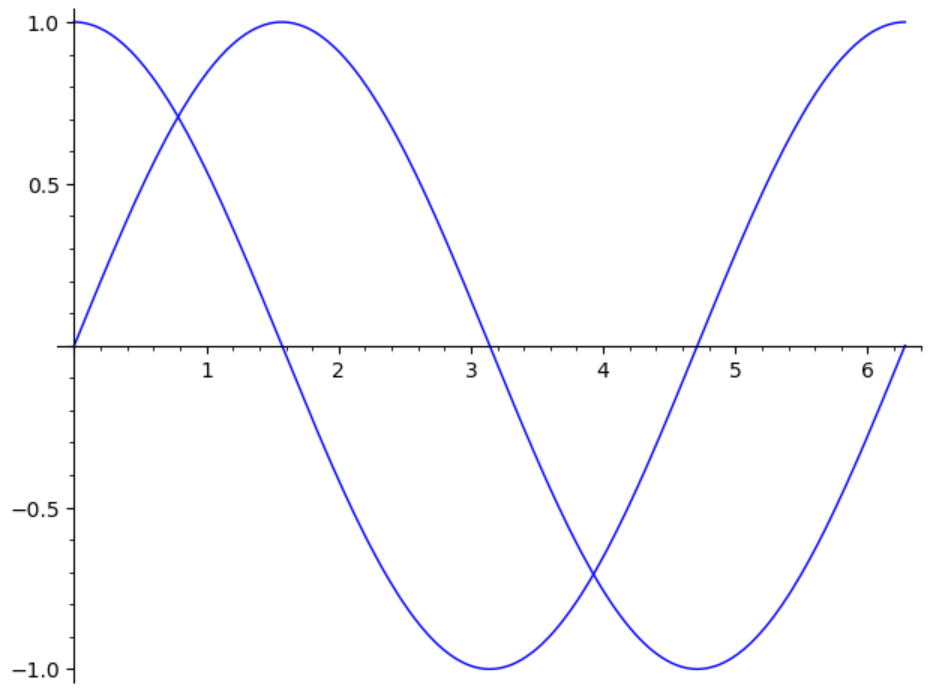
\includegraphics[width=0.5\linewidth]{images/screenshot009}
	\caption{Đồ thị với cả hai hàm \(\sin(x)\) và \(\cos(x)\) trên cùng một biểu đồ}
	\label{fig:screenshot009}
\end{figure}

\subsubsection{Vẽ đồ thị 3D của hàm số}

SageMath cũng cho phép vẽ đồ thị 3D của các hàm hai biến. Để vẽ đồ thị 3D, bạn có thể sử dụng hàm \texttt{plot3d}. Ví dụ, vẽ đồ thị của hàm \( f(x, y) = \sin(x^2 + y^2) \):

\begin{lstlisting}
	sage: plot3d(sin(x^2 + y^2), (x, -3, 3), (y, -3, 3))  # Ve do thi 3D cua ham sin(x^2 + y^2)
\end{lstlisting}
\begin{figure}
	\centering
	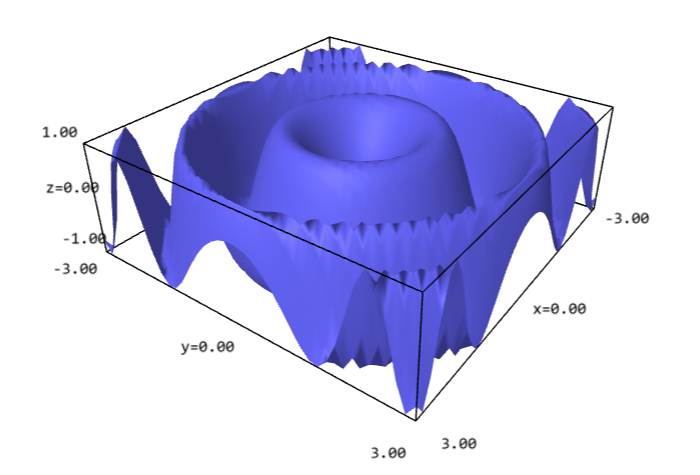
\includegraphics[width=0.7\linewidth]{images/screenshot010}
	\caption{Một bề mặt 3D của hàm \( \sin(x^2 + y^2) \) trong khoảng \([-3, 3]\) cho cả \(x\) và \(y\)}
	\label{fig:screenshot010}
\end{figure}

\subsubsection{Tùy chỉnh đồ thị}

SageMath cung cấp nhiều tùy chọn để tùy chỉnh đồ thị, chẳng hạn như thay đổi màu sắc, thêm tiêu đề, điều chỉnh trục, hoặc thay đổi độ dày đường nét. Các tùy chọn này có thể giúp bạn tạo ra các biểu đồ trực quan và dễ hiểu hơn.

Ví dụ, vẽ đồ thị của hàm \( f(x) = e^x \) và thêm tiêu đề, nhãn trục:

\begin{lstlisting}
	# Ve do thi ham so exp(x) voi tieu de va nhan
	sage: p = plot(exp(x), (x, 0, 5), color='green')
	sage: p.axes_labels(['x', 'exp(x)'])
	sage: p.show(title='Graph of exp(x)')
\end{lstlisting}
\begin{figure}
	\centering
	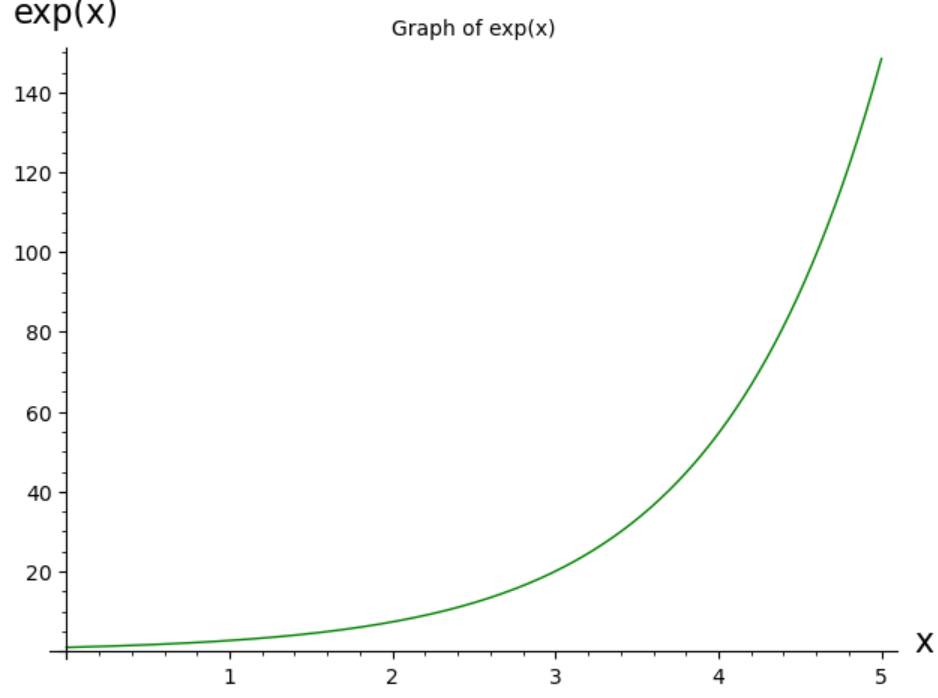
\includegraphics[width=0.7\linewidth]{images/screenshot011}
	\caption{Đồ thị của \( e^x \) với màu xanh lá, thêm tiêu đề cùng với nhãn cho các trục}
	\label{fig:screenshot011}
\end{figure}

\subsubsection{Vẽ đồ thị parametric}

SageMath cũng hỗ trợ vẽ đồ thị các hàm parametric. Các hàm parametric được định nghĩa bởi một cặp hàm số \( x(t) \) và \( y(t) \), với \( t \) là tham số. Ví dụ, vẽ đồ thị của đường tròn với bán kính \(r = 1\):

\begin{lstlisting}
	sage: var('t')	#Khai bao bien t
	sage: parametric_plot([cos(t), sin(t)], (t, 0, 2*pi))  # Ve do thi cua duong tron
\end{lstlisting}
\begin{figure}
	\centering
	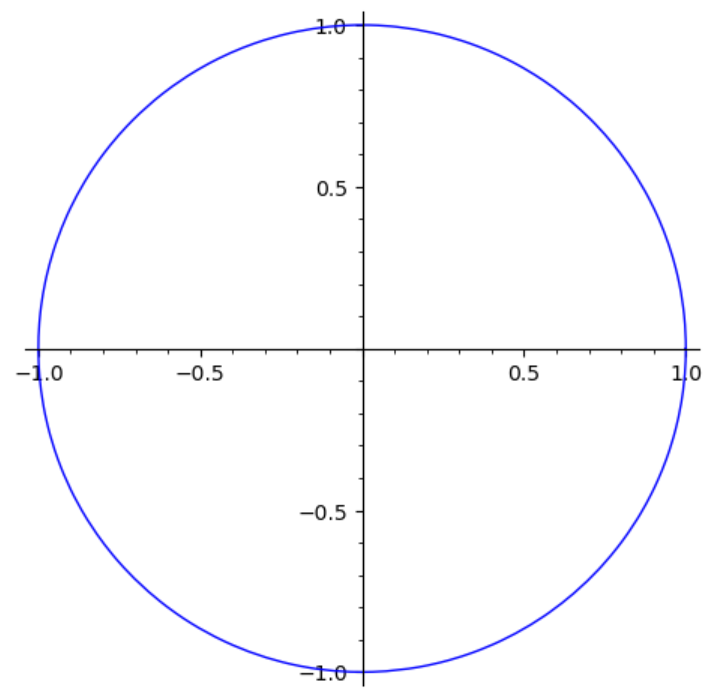
\includegraphics[width=0.7\linewidth]{images/screenshot012}
	\caption{Đồ thị của một đường tròn đơn vị trong mặt phẳng \( Oxy \)}
	\label{fig:screenshot012}
\end{figure}

\section{Tổ hợp, xác suất và logic}
\subsection{Tính toán tổ hợp, xác suất và thống kê}

SageMath cung cấp một bộ công cụ mạnh mẽ để làm việc với các vấn đề tổ hợp, xác suất và thống kê. Phần này sẽ giới thiệu cách sử dụng SageMath để thực hiện các phép toán tổ hợp, tính xác suất và xử lý các bài toán thống kê.

\subsubsection{Tính toán tổ hợp}

Trong tổ hợp, các phép toán như chèn chỗ và kết hợp được sử dụng để tính toán số cách chọn một tập hợp con từ một tập hợp lớn hơn. SageMath cung cấp các hàm như \texttt{binomial} và \texttt{factorial} để tính các giá trị tổ hợp, chỉnh hợp và giai thừa.

Ví dụ, tính số cách chọn 3 phần tử từ một tập hợp 5 phần tử:

\begin{lstlisting}
	sage: binomial(5, 3)  # Tinh to hop chap 3 cua 5
	10
\end{lstlisting}

Ví dụ, tính số cách chọn và sắp xếp 3 phần tử từ một tập hợp 5 phần tử:
\begin{lstlisting}
	sage: permutation(5, 3)  # Tinh chinh hop 3 cua 5
	60
\end{lstlisting}

Ngoài ra, bạn có thể tính giai thừa của một số bằng cách sử dụng hàm \texttt{factorial}:

\begin{lstlisting}
	sage: factorial(5)  # Tinh 5!
	120
\end{lstlisting}

\subsubsection{Tính toán xác suất}

SageMath hỗ trợ tính toán xác suất trong các bài toán tổ hợp. Để tính xác suất, bạn có thể sử dụng các hàm như \texttt{probability}, \texttt{random}, và các hàm xác suất phân phối.

Ví dụ, tính xác suất để một con xúc xắc ra mặt 6:

\begin{lstlisting}
	sage: P = 1/6  # Xac suat ra mat 6
	P
	1/6
\end{lstlisting}

SageMath cung cấp hàm \texttt{probability} để tính toán xác suất trong các bài toán phức tạp hơn, đặc biệt khi làm việc với các phân phối xác suất. Ví dụ, ta có thể tính xác suất của một sự kiện trong một không gian mẫu xác định, chẳng hạn xác suất để lăn xúc xắc và ra mặt 6:

\begin{lstlisting}
	sage: P = probability(lambda: random_integer(1, 6) == 6)  # Xac suat ra mat 6
	P
	1/6
\end{lstlisting}

SageMath cũng hỗ trợ việc tạo các giá trị ngẫu nhiên từ phân phối xác suất. Ví dụ, để tạo một giá trị ngẫu nhiên từ phân phối đồng đều trên khoảng từ 1 đến 6 (giống như lăn xúc xắc), bạn có thể sử dụng hàm \texttt{random\_integer}:

\begin{lstlisting}
	sage: random_integer(1, 6)  # Sinh so ngau nhien giua 1 va 6
\end{lstlisting}

Hàm \texttt{random\_integer(a, b)} sẽ trả về một giá trị ngẫu nhiên trong khoảng từ \(a\) đến \(b\), bao gồm cả \(a\) và \(b\).

Bạn cũng có thể tính xác suất của các sự kiện phức tạp hơn, chẳng hạn như xác suất ra mặt chẵn khi lăn một con xúc xắc. Sử dụng hàm \texttt{probability} với một điều kiện phức tạp:

\begin{lstlisting}
	sage: P_even = probability(lambda: random_integer(1, 6) in [2, 4, 6])  # Xac suat ra mat chan
	P_even
	1/2
\end{lstlisting}

Ở đây, chúng ta đã tính xác suất ra mặt chẵn của con xúc xắc. Kết quả xác suất là \( \frac{3}{6} = \frac{1}{2} \), vì có ba mặt chẵn (2, 4, 6) trong tổng số sáu mặt của xúc xắc.

\subsubsection{Phân phối xác suất}

SageMath hỗ trợ nhiều loại phân phối xác suất, bao gồm phân phối nhị thức, phân phối chuẩn và phân phối Poisson. Bạn có thể sử dụng các hàm như\\ \texttt{binomial\_distribution}, \texttt{normal\_distribution}, và \texttt{poisson\_distribution} để làm việc với các phân phối này.

Ví dụ, tính xác suất để có ít nhất 3 mặt "được" trong 5 lần gieo xúc xắc với phân phối nhị thức:

\begin{lstlisting}
	sage: B = binomial_distribution(5, 1/6)  # Phan phoi nhi thuc cho 5 lan gieo
	P = B.cdf(3)  # Cumulative distribution function de tinh xac suat co it nhat 3 lan "duoc"
	P
	0.868050607
\end{lstlisting}

\subsubsection{Tính toán thống kê}

SageMath cũng cung cấp các công cụ mạnh mẽ để tính toán thống kê mô tả như trung bình, phương sai, độ lệch chuẩn và các phép toán thống kê khác.

Ví dụ, tính trung bình và độ lệch chuẩn của một dãy số:

\begin{lstlisting}
	sage: data = [12, 15, 20, 25, 30, 35, 40]
	sage: mean(data)  # Tinh trung binh
	25.2857142857143
	sage: stdev(data)  # Tinh do lech chuan
	9.49460415914107
\end{lstlisting}

Các hàm \texttt{mean} và \texttt{stdev} tính toán trung bình và độ lệch chuẩn của dãy số.

\subsubsection{Kiểm định giả thuyết}

SageMath cung cấp các công cụ để thực hiện các kiểm định giả thuyết thống kê. Ví dụ, kiểm định t-Student để kiểm tra sự khác biệt giữa trung bình mẫu và trung bình giả thuyết.

Ví dụ, thực hiện kiểm định t với dãy số và trung bình giả thuyết là 25:

\begin{lstlisting}
	sage: t_test(data, 25)  # Kiem dinh t voi trung binh gia thuyet 25
	(0.285714285714286, 0.781595168902066)
\end{lstlisting}

Kết quả trả về là giá trị thống kê t và giá trị p. Với giá trị p này, bạn có thể quyết định có bác bỏ giả thuyết hay không.


\subsection{Làm việc với số học rời rạc và lý thuyết số}

SageMath cung cấp các công cụ rất mạnh mẽ để làm việc với số học rời rạc và lý thuyết số, cho phép thực hiện từ những thao tác đơn giản như tính \texttt{mod}, kiểm tra nguyên tố đến những thao tác phức tạp hơn như định lý phần dư Trung Hoa, logarit rời rạc, và hệ thống số học hữu hạn.

\subsubsection{Số nguyên tố và kiểm tra nguyên tố}

Bạn có thể dễ dàng tạo danh sách các số nguyên tố hoặc kiểm tra một số có phải nguyên tố hay không bằng các hàm \texttt{is\_prime}, \texttt{next\_prime}, \texttt{prime\_pi}, và \texttt{primes}.

\begin{lstlisting}
	sage: is_prime(37)
	True
	sage: next_prime(100)
	101
	sage: primes(50, 70)
	[53, 59, 61, 67]
\end{lstlisting}

\subsubsection{Ước số chung lớn nhất và bội số chung nhỏ nhất}

SageMath hỗ trợ tính ước số chung lớn nhất (GCD) và bội số chung nhỏ nhất (LCM) bằng các hàm \texttt{gcd} và \texttt{lcm}.

\begin{lstlisting}
	sage: gcd(48, 180)
	12
	sage: lcm(12, 18)
	36
\end{lstlisting}

\subsubsection{Số học modulo}

Số học modulo là nền tảng trong nhiều thuật toán lý thuyết số. Bạn có thể sử dụng toán tử \texttt{\%} hoặc tạo trường số dư với \texttt{Zmod(n)}.

\begin{lstlisting}
	sage: 17 % 5
	2
	sage: R = Zmod(7)
	sage: a = R(3)
	sage: b = R(5)
	sage: a * b
	R(1)
\end{lstlisting}

\subsubsection{Định lý phần dư Trung Hoa}

SageMath hỗ trợ định lý phần dư Trung Hoa qua hàm \texttt{crt} để tìm số thỏa mãn một hệ phương trình đồng dư.

\begin{lstlisting}
	sage: crt([2, 3, 2], [3, 5, 7])  # Chinese Remainder Theorem
	23
\end{lstlisting}

\subsubsection{Hàm Euler và số nguyên tố cùng nhau}

Hàm Euler \(\phi(n)\) đếm số nguyên nhỏ hơn \(n\) nguyên tố cùng nhau với \(n\). SageMath cung cấp hàm \texttt{euler\_phi} và \texttt{is\_coprime} để làm việc với tính chất này.

\begin{lstlisting}
	sage: euler_phi(10)
	4
	sage: gcd(7, 10) == 1  # 7 and 10 are coprime
	True
\end{lstlisting}

\subsubsection{Lũy thừa modulo và logarit rời rạc}

Phép toán lũy thừa modulo có thể được thực hiện hiệu quả với hàm \texttt{power\_mod}, và SageMath cũng hỗ trợ tìm logarit rời rạc trong một số trường hợp.

\begin{lstlisting}
	sage: power_mod(3, 4, 5)
	1
	sage: Z5 = Zmod(5)
	sage: Z5(3).log(2)  # Solve 2^x = 3 mod 5
	3
\end{lstlisting}

\subsubsection{Trường số và phần tử đại số}

SageMath cho phép bạn tạo và làm việc với các trường số (number fields), ví dụ trường chứa căn bậc hai hoặc các phần tử đại số khác.

\begin{lstlisting}
	sage: K.<a> = NumberField(x^2 - 2)
	sage: a^2
	2
\end{lstlisting}


\subsection{Tính toán với tập hợp, logic và điều kiện}

SageMath hỗ trợ nhiều công cụ để thao tác với tập hợp, biểu thức logic và điều kiện. Các cấu trúc này không chỉ hữu ích trong toán học rời rạc mà còn trong việc xây dựng mô hình, tự động hóa kiểm định mệnh đề và viết mã có điều kiện.

\subsubsection{Tập hợp và các phép toán trên tập hợp}

Bạn có thể định nghĩa các tập hợp và thực hiện các phép toán như hợp, giao, hiệu, hiệu đối xứng và kiểm tra phần tử.

\begin{lstlisting}
	sage: A = Set([1, 2, 3, 4])
	sage: B = Set([3, 4, 5, 6])
	sage: A.union(B)
	{1, 2, 3, 4, 5, 6}
	sage: A.intersubsection(B)
	{3, 4}
	sage: A.difference(B)
	{1, 2}
	sage: A.symmetric_difference(B)
	{1, 2, 5, 6}
	sage: 3 in A
	True
\end{lstlisting}

Ngoài ra, SageMath còn hỗ trợ tập rỗng, tập vô hạn, tập định nghĩa bằng điều kiện và các tập số học đặc biệt như tập số nguyên, tập số thực, tập hữu tỷ, \dots

\begin{lstlisting}
	sage: EmptySet()
	{}
	sage: QQ.is_subset(RR)
	True
\end{lstlisting}

\subsubsection{Biểu thức logic và phép toán mệnh đề}

SageMath cho phép tạo và đánh giá các biểu thức logic sử dụng các phép toán: \texttt{and}, \texttt{or}, \texttt{not}, \texttt{xor}, \texttt{implies}, \texttt{iff}.

\begin{lstlisting}
	sage: a, b = var('a b')
	sage: f = a & ~b
	sage: f.simplify_logic()
	a & ~b
\end{lstlisting}

Bạn cũng có thể kiểm tra tính đúng sai hoặc tương đương logic giữa các biểu thức.

\begin{lstlisting}
	sage: f1 = (a & b) | (~a & b)
	sage: f2 = b
	sage: bool(f1.simplify_logic() == f2.simplify_logic())
	True
\end{lstlisting}

\subsubsection{Câu lệnh điều kiện \texttt{if} và các biểu thức điều kiện}

Trong khi SageMath chủ yếu dùng cho biểu thức toán học, nó cũng hỗ trợ biểu thức điều kiện trong mã Python:

\begin{lstlisting}
	sage: x = 5
	sage: if x % 2 == 0:
	....:     y = "even"
	....: else:
	....:     y = "odd"
	sage: y
	'odd'
\end{lstlisting}

Bạn có thể dùng biểu thức điều kiện ngắn gọn dạng \texttt{a if condition else b}:

\begin{lstlisting}
	sage: z = "positive" if x > 0 else "non-positive"
	sage: z
	'positive'
\end{lstlisting}

\subsubsection{Mệnh đề định lượng: forall và exists}

Trong SageMath, việc biểu diễn các lượng từ toán học (\texttt{forall}, \texttt{exists}) không được hỗ trợ trực tiếp thông qua các hàm \texttt{ForAll} và \texttt{Exists} như trong một số ngôn ngữ lập trình khác. Thay vào đó, chúng ta có thể sử dụng các phương pháp kiểm tra tính đúng của mệnh đề bằng cách sử dụng các hàm kiểm tra giá trị cụ thể hoặc dùng giả thuyết với hàm \texttt{assume()}.

\textbf{Ví dụ:} Kiểm tra mệnh đề với tập giá trị hữu hạn

\begin{lstlisting}
	# Kiem tra dieu kien x^2 >= 0 voi cac gia tri cu the
	sage: x = var('x')
	sage: all((x^2 >= 0) for x in [-10, -1, 0, 1, 10])
	# Ket qua: True
\end{lstlisting}

\textbf{Ví dụ:} Kiểm tra với giả thuyết

\begin{lstlisting}
	# Kiem tra dieu kien voi gia thuyet x la so thuc
	sage: assume(x, 'real')
	sage: bool(x^2 >= 0)
	# Ket qua: True
\end{lstlisting}

	
	% Chương 4: Các tính năng nâng cao và tùy chỉnh
	\chapter{Các tính năng nâng cao và tùy chỉnh}
	\section{Lập trình trong SageMath bằng Python}
	
SageMath được xây dựng dựa trên Python, cho phép người dùng sử dụng đầy đủ các cấu trúc điều khiển, hàm, lớp và thư viện của ngôn ngữ này. Điều này giúp mở rộng khả năng xử lý và tạo ra các chương trình toán học linh hoạt.

\subsection{Câu lệnh điều kiện và vòng lặp}
Người dùng có thể sử dụng các cấu trúc điều kiện như \texttt{if-else} và vòng lặp như \texttt{for}, \texttt{while} trong SageMath.

\begin{lstlisting}[basicstyle=\ttfamily\small]
	# Kiem tra so nguyen to bang cau lenh if
	sage: def is_prime_check(n):
	....:     if is_prime(n):
	....:         return "La so nguyen to"
	....:     else:
	....:         return "Khong la so nguyen to"
	
	sage: is_prime_check(17)
	'La so nguyen to'
	
	# Duyet cac so nguyen to nho hon 20
	sage: for i in range(1, 20):
	....:     if is_prime(i):
	....:         print(i)
	2
	3
	5
	7
	11
	13
	17
	19
\end{lstlisting}

\subsection{Định nghĩa và sử dụng hàm}
Người dùng có thể định nghĩa hàm tùy chỉnh trong SageMath tương tự như trong Python.

\begin{lstlisting}[basicstyle=\ttfamily\small]
	# Ham tinh giai thua bang de quy
	sage: def giaithua(n):
	....:     if n == 0:
	....:         return 1
	....:     else:
	....:         return n * giaithua(n - 1)
	
	sage: giaithua(5)
	120
\end{lstlisting}

\subsection{Làm việc với danh sách và tập hợp}
Các cấu trúc dữ liệu như danh sách, tập hợp, từ điển... đều có thể sử dụng trong SageMath để xử lý dữ liệu toán học linh hoạt.

\begin{lstlisting}[basicstyle=\ttfamily\small]
	# Tao danh sach cac binh phuong
	sage: squares = [n^2 for n in range(1, 11)]
	sage: squares
	[1, 4, 9, 16, 25, 36, 49, 64, 81, 100]
	
	# Tap hop cac uoc so cua 24
	sage: divisors(24)
	[1, 2, 3, 4, 6, 8, 12, 24]
\end{lstlisting}

\subsection{Sử dụng lambda và biểu thức hàm}
Biểu thức lambda giúp định nghĩa hàm ngắn gọn và kết hợp với các hàm bậc cao như \texttt{map}, \texttt{filter}, \texttt{reduce}.

\begin{lstlisting}[basicstyle=\ttfamily\small]
	# Su dung lambda de tinh lap phuong
	sage: lap_phuong = lambda x: x^3
	sage: lap_phuong(4)
	64
	
	# Loc cac so chia het cho 3
	sage: list(filter(lambda x: x % 3 == 0, range(1, 20)))
	[3, 6, 9, 12, 15, 18]
\end{lstlisting}

Như vậy, SageMath không chỉ là công cụ toán học mạnh mẽ mà còn là môi trường lập trình tiện lợi, linh hoạt với đầy đủ sức mạnh của Python.

\section{SageMath trong tính toán khoa học}
	
SageMath không chỉ là công cụ tính toán toán học thuần túy mà còn được sử dụng rộng rãi trong tính toán khoa học (scientific computing), nhờ tích hợp với các thư viện nổi tiếng như NumPy, SciPy và matplotlib.

\subsection{Sử dụng NumPy để xử lý mảng số liệu}

SageMath hỗ trợ thư viện NumPy để thao tác với mảng và thực hiện các phép toán số học hiệu quả.

\begin{lstlisting}[basicstyle=\ttfamily\small]
	# Tao mang numpy va tinh tong
	sage: import numpy as np
	sage: a = np.array([1, 2, 3, 4])
	sage: b = np.array([10, 20, 30, 40])
	sage: a + b
	array([11, 22, 33, 44])
\end{lstlisting}

\subsection{Sử dụng SciPy để giải bài toán khoa học}

SciPy cung cấp nhiều công cụ để giải phương trình, tích phân, tối ưu hóa và các bài toán vật lý kỹ thuật.

\begin{lstlisting}[basicstyle=\ttfamily\small]
	# Tim nghiem gan dung cua phuong trinh
	sage: from scipy.optimize import fsolve
	sage: f = lambda x: x**3 - 1
	sage: fsolve(f, 0.5)
	array([1.])
\end{lstlisting}

\subsection{Vẽ đồ thị khoa học với matplotlib}

SageMath có thể dùng matplotlib để tạo các biểu đồ trực quan hóa dữ liệu.

\begin{lstlisting}[basicstyle=\ttfamily\small]
	# Ve do thi ham sin(x)
	sage: import matplotlib.pyplot as plt
	sage: import numpy as np
	sage: x = np.linspace(0, 2*np.pi, 100)
	sage: y = np.sin(x)
	sage: plt.plot(x, y)
	sage: plt.title('Do thi sin(x)')
	sage: plt.grid()
	sage: plt.show()
\end{lstlisting}
\begin{figure}[H]
	\centering
	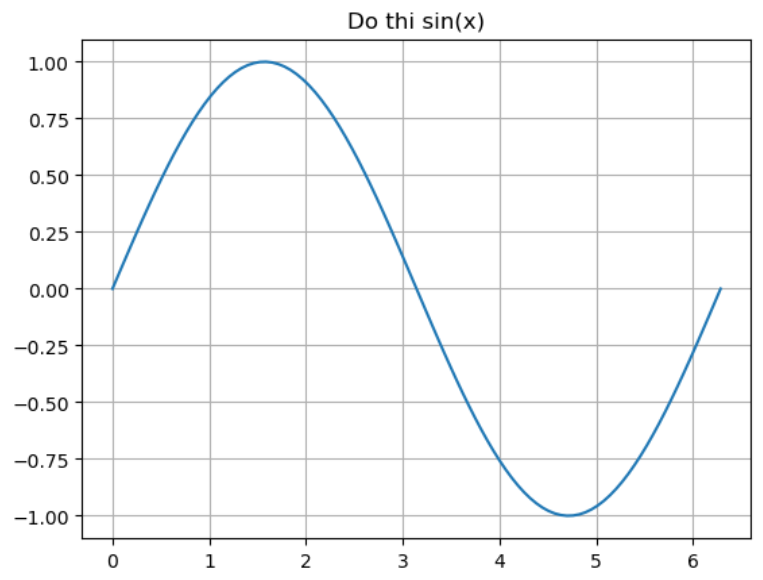
\includegraphics[width=0.7\linewidth]{images/4232}
	\caption{Vẽ đồ thị $y=sin(x)$ trên đoạn $\left[0,2\pi\right]$ với matplotlib}
	\label{fig:4232}
\end{figure}


Nhờ tích hợp tốt với các công cụ khoa học hiện đại, SageMath cho phép người dùng thực hiện các bài toán từ lý thuyết đến ứng dụng kỹ thuật một cách hiệu quả.

\section{Mở rộng SageMath với thư viện bên ngoài}

Một trong những điểm mạnh của SageMath là khả năng mở rộng thông qua các thư viện bên ngoài, đặc biệt là các thư viện của Python. Người dùng có thể dễ dàng cài đặt và sử dụng các gói bổ sung để tăng cường chức năng của SageMath.

\subsection{Cài đặt thư viện bổ sung}

Người dùng có thể cài đặt các thư viện Python bằng lệnh \texttt{pip} ngay trong SageMath:

\begin{lstlisting}[basicstyle=\ttfamily\small]
	# Cai thu vien sympy
	sage: !pip install sympy
\end{lstlisting}

Sau khi cài đặt, ta có thể nhập và sử dụng ngay:

\begin{lstlisting}[basicstyle=\ttfamily\small]
	# Su dung sympy de rut gon bieu thuc
	sage: import sympy as sp
	sage: x = sp.Symbol('x')
	sage: expr = (x**2 + 2*x + 1)/(x + 1)
	sage: sp.simplify(expr)
	x + 1
\end{lstlisting}

\subsection{Kết hợp SageMath với pandas để xử lý dữ liệu}

Pandas là một thư viện mạnh để thao tác với dữ liệu dạng bảng.

\begin{lstlisting}[basicstyle=\ttfamily\small]
	# Doc file CSV va thong ke
	sage: import pandas as pd
	sage: data = pd.read_csv('du_lieu.csv')
	sage: data.head()
	sage: data.describe()
\end{lstlisting}

\subsection{Sử dụng thư viện tính toán nâng cao}

Một số thư viện khác có thể dùng để xử lý các bài toán đặc biệt như:

\begin{itemize}
	\item \textbf{networkx} – phân tích đồ thị và mạng.
	\item \textbf{scikit-learn} – học máy cơ bản.
	\item \textbf{cvxpy} – tối ưu hóa lồi.
\end{itemize}

Ví dụ dùng \texttt{networkx} để tạo đồ thị:

\begin{lstlisting}[basicstyle=\ttfamily\small]
	# Tao do thi bang networkx
	sage: import networkx as nx
	sage: G = nx.Graph()
	sage: G.add_edges_from([(1, 2), (2, 3), (3, 1)])
	sage: nx.draw(G, with_labels=True)
\end{lstlisting}

\begin{figure}[H]
	\centering
	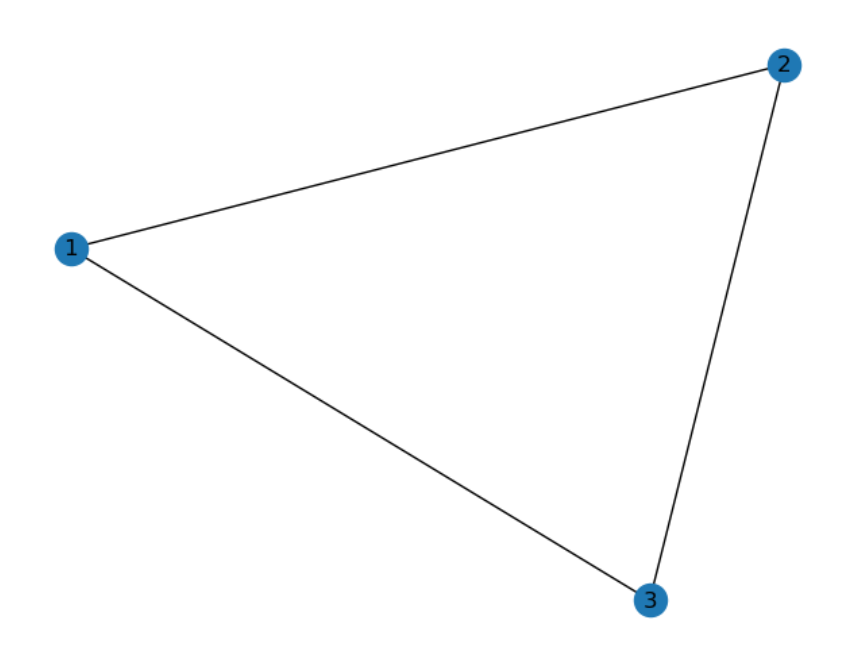
\includegraphics[width=0.45\linewidth]{images/423}
	\caption{Đồ thị được tạo bằng networkx}
	\label{fig:423}
\end{figure}


Khả năng mở rộng giúp SageMath trở thành nền tảng mở, thân thiện với nghiên cứu và giảng dạy hiện đại.

\newpage
\section{Kết nối SageMath với các phần mềm khác}

SageMath có thể tích hợp với nhiều phần mềm và hệ thống khác để phục vụ các mục đích đa dạng như trình bày tài liệu, xử lý dữ liệu, và phát triển ứng dụng.

\subsection{Sử dụng SageMath với \LaTeX{}}

SageMath hỗ trợ tích hợp trực tiếp với \LaTeX{} thông qua gói \texttt{sagetex}. Gói này cho phép người dùng chèn mã SageMath vào file \LaTeX{} và tự động sinh kết quả.

Ví dụ: file \texttt{main.tex} chứa đoạn sau:

\begin{lstlisting}[basicstyle=\ttfamily\small]
	\documentclass{article}
	\usepackage{sagetex}
	\begin{document}
		Gia tri cua $f(x) = x^2 + 1$ tai $x = 3$ la \sage{3^2 + 1}.
	\end{document}
\end{lstlisting}

Sau khi biên dịch bằng \texttt{pdflatex} và chạy mã Sage, kết quả sẽ tự động được chèn vào văn bản.

\subsection{Kết nối với Jupyter Notebook}

SageMath có thể chạy trong môi trường Jupyter Notebook – nơi cho phép người dùng viết mã, hiển thị công thức, hình ảnh và chú thích trong cùng một giao diện tương tác.

\begin{lstlisting}[basicstyle=\ttfamily\small]
	# Chay Sage trong Jupyter Notebook
	$ sage -n jupyter
\end{lstlisting}

Người dùng có thể dễ dàng thao tác các biểu thức toán học, vẽ đồ thị và phân tích dữ liệu trực tiếp trong các ô (cell).

\subsection{Tích hợp với Python IDE}

Vì SageMath là một lớp bao ngoài của Python, ta có thể dùng SageMath trong các môi trường lập trình như VSCode hoặc PyCharm với một chút thiết lập. Điều này giúp phát triển các ứng dụng lớn và chuyên sâu hơn.

\subsection{Giao tiếp với phần mềm toán học khác}

SageMath còn có thể giao tiếp với các phần mềm khác như:

\begin{itemize}
	\item \textbf{R} – phân tích thống kê.
	\item \textbf{Mathematica, Maple} – chuyển đổi định dạng.
	\item \textbf{Maxima, GAP, Singular} – tích hợp trong nội bộ SageMath.
\end{itemize}

Ví dụ gọi Maxima trong Sage:

\begin{lstlisting}[basicstyle=\ttfamily\small]
	# Goi Maxima de rut gon bieu thuc
	sage: maxima('(x^2 + 2*x + 1)/(x + 1)').ratsimp()
	x + 1
\end{lstlisting}

Tính linh hoạt trong tích hợp giúp SageMath dễ dàng được đưa vào hệ sinh thái học thuật, nghiên cứu và công nghiệp.


	
	% Chương 5: Ứng dụng trong các học phần Toán đại cương
	\chapter{Ứng dụng trong các học phần Toán đại cương}
	\section{Ứng dụng trong Giải tích 1}

\subsection{Phép tính vi phân hàm một biến số}

\subsubsection{Tìm tập xác định của hàm số}

Xét hàm số \( y = \sqrt{2\ln{x} - 3} \). Điều kiện xác định là biểu thức trong hàm $\ln$ phải dương và biểu thức trong căn phải không âm:
\[
\left\{
\begin{aligned}
	&x > 0 \\
	&2\ln{x} - 3 \geq 0 \Rightarrow \ln{x} \geq \frac{3}{2} \Rightarrow x \geq e^{\frac{3}{2}}
\end{aligned}
\right.
\]

Giải điều kiện trong SageMath:
\begin{lstlisting}
	sage: var('x')
	sage: solve(log(x) >= 3/2, x)
	[x >= e^(3/2)]
\end{lstlisting}

Vậy tập xác định của hàm là $D=\left[e^{\frac{3}{2}};+\infty \right)$.

\textbf{Lưu ý:} Hàm \texttt{solve()} trong SageMath có thể trả về kết quả dưới dạng các biểu thức logic hoặc bất phương trình, và bạn có thể áp dụng các hàm như \texttt{find\_root()} hoặc \texttt{plot()} để kiểm tra trực quan kết quả. 

\subsubsection{Tìm miền giá trị của hàm số}

Xét hàm số \( y = \sqrt{1 - \left( \frac{x - 1}{x + 1} \right)^2} \). Tìm miền giá trị của hàm số trên tập (0;2).

\begin{lstlisting}
	sage: var('x')
	sage: f(x) = sqrt(1 - ((x - 1)/(x + 1))^2)
	sage: f.find_local_maximum(0, 2)
	(1.00000000000000, 0.999999967094019)
	sage: f.find_local_minimum(0, 2)
	(0.0001869787205816002, 8.740260678362169e-09)
\end{lstlisting}

Kết quả cho biết trên tập (0;2), tập giá trị của $f(x)$ là \\$(8.740260678362169e-09, 0.999999967094019)
$.

\subsubsection{Làm việc với hàm hyperbolic}
Ví dụ hàm \( f(x) = \sinh(x) + \cosh(x) \):
\begin{lstlisting}
	sage: f(x) = sinh(x) + cosh(x)
	sage: f(1)
	cosh(1) + sinh(1)
	sage: float(f(1))
	2.718281828459045
\end{lstlisting}

\subsubsection{Tìm hàm \( f(x) \)}
Tìm hàm $f(x)$, biết \( f(x + \frac{1}{x}) = x^2 + \frac{1}{x^2} \).\\

Gợi ý biến đổi biểu thức: Đặt \( t = x + \frac{1}{x} \Rightarrow f(t) = t^2 - 2 \).
\begin{lstlisting}
	sage: var('x t')
	sage: t = x + 1/x
	sage: expr = x^2 + 1/x^2
	sage: f_t = simplify((t)^2 - 2)
	sage: f_t
	(x + 1/x)^2 - 2
\end{lstlisting}

\subsubsection{Tìm hàm ngược}

Cho hàm \( y = \frac{1}{2}(e^x - e^{-x}) = \sinh(x) \). Hàm ngược của hàm số này là \( x = \operatorname{arcsinh}(y) \), hay còn gọi là hàm sinh ngược.

Giải phương trình để tìm hàm ngược trong SageMath:

\begin{lstlisting}
	sage: var('x y')
	sage: solve(y == (1/2)*(exp(x) - exp(-x)), x)
	[x == log(y - sqrt(y^2 + 1)), x == log(y + sqrt(y^2 + 1))]
\end{lstlisting}

Kết quả SageMath trả về là:

\[
x = \ln\left( y + \sqrt{y^2 + 1} \right)
\]

Do đó, hàm ngược là:

\[
\boxed{f^{-1}(y) = \ln\left( y + \sqrt{y^2 + 1} \right)}
\]

\subsubsection{Tính giới hạn, kiểm tra tính liên tục}
Xét hàm \( f(x) = \frac{x}{4 - x^2} \) trên khoảng \( [-1,1] \).

Giới hạn tại biên:
\begin{lstlisting}
	sage: limit(x/(4 - x^2), x=1)
	1/3
	sage: limit(x/(4 - x^2), x=-1)
	-1/3
\end{lstlisting}

\subsubsection{Tính đạo hàm, cực trị, tiệm cận}
Cho hàm \( y = x - \ln(1 + x) \):
\begin{lstlisting}
	   sage: f(x) = x - log(1 + x)
	sage: diff(f, x)              # Dao ham cap 1
	x |--> -1/(x + 1) + 1
	sage: diff(f, x, 2)           # Dao ham cap 2
	x |--> (x + 1)^(-2)
	sage: solve(diff(f, x) == 0, x)  # Tim cuc tri
	[x == 0]
	sage: limit(f, x=-oo)	# Tiem can ngang (Gioi han trai)
	x |--> -Infinity
	sage: limit(f, x=+oo)	# Tiem can ngang (Gioi han phai)
	x |--> +Infinity
	sage: limit(f, x=-1)          # Tiem can dung
	x |--> Infinity
\end{lstlisting}

\subsection{Phép tính tích phân hàm một biến số}

\subsubsection{Tính tích phân bất định}
\begin{lstlisting}
	sage: integrate(tan(x)^3, x)
	-1/2/(sin(x)^2 - 1) + 1/2*log(sin(x)^2 - 1)
\end{lstlisting}

\subsubsection{Tính tích phân xác định}
\begin{lstlisting}
	sage: integrate(exp(-x^2), (x, -1, 1))
	sqrt(pi)*erf(1)
\end{lstlisting}

\subsubsection{Tính tích phân suy rộng}
\begin{lstlisting}
	sage: integrate(1/x^2, (x, 1, oo))
	1
\end{lstlisting}

\subsubsection{Tính diện tích hình phẳng}
Diện tích giữa đồ thị \( y = \sin{x} \) và trục hoành từ \( 0 \) đến \( \pi \):
\begin{lstlisting}
	sage: integrate(abs(sin(x)), (x, 0, pi))
	2
\end{lstlisting}

\subsubsection{Thể tích vật thể quay quanh trục hoành}
Cho \( y = \sqrt{x} \), thể tích khi quay quanh trục $Ox$ từ 0 đến 1:
\begin{lstlisting}
	sage: integrate(pi * (sqrt(x))^2, (x, 0, 1))
	1/2*pi
\end{lstlisting}

\subsection{Hàm số nhiều biến số}

\subsubsection{Tính giới hạn hàm nhiều biến}
SageMath không tự động tính giới hạn nhiều biến tại điểm như Mathematica hay Maple.

\subsubsection{Đạo hàm riêng và vi phân toàn phần}
Xét hàm \( f(x, y) = \frac{x^2 y}{x^2 + y^2} \):
\begin{lstlisting}
	sage: var('x y')
	sage: f(x, y) = (x^2 * y)/(x^2 + y^2)
	sage: diff(f, x)	# Dao ham theo bien x
	(x, y) |--> -2*x^3*y/(x^2 + y^2)^2 + 2*x*y/(x^2 + y^2)
	sage: diff(f, y)	# Dao ham theo bien y
	(x, y) |--> -2*x^2*y^2/(x^2 + y^2)^2 + x^2/(x^2 + y^2)
\end{lstlisting}

Kết quả là:
$$f'_x(x,y)=\dfrac{-2x^3y}{x^2 + y^2}+\dfrac{2xy}{x^2 + y^2}$$
$$f'_y(x,y)=\dfrac{-2x^2y^2}{x^2 + y^2}+\dfrac{x^2}{x^2 + y^2}$$

\subsubsection{Khai triển chuỗi Taylor-Maclaurin hàm nhiều biến}
Xét hàm \( f(x, y) =  e^{x+y}\):
\begin{lstlisting}
	sage: var('x y')
	sage: f(x, y) = exp(x + y)
	sage: taylor(f, (x, 0), 3)
	(x, y) |--> 1/6*x^3*e^y + 1/2*x^2*e^y + x*e^y + e^y
\end{lstlisting}

Kết quả là: $\frac{1}{6}x^3e^y + \frac{1}{2}x^2e^y + xe^y + e^y$.

\subsubsection{Vẽ đồ thị hàm số nhiều biến}
\begin{lstlisting}
	sage: var('x y')
	sage: plot3d(sin(x^2 + y^2), (x, -2, 2), (y, -2, 2))
\end{lstlisting}
\begin{figure}[H]
	\centering
	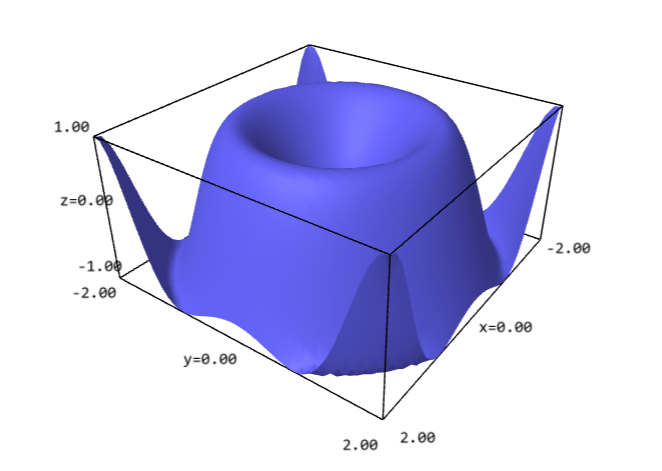
\includegraphics[width=0.7\linewidth]{images/5134}
	\caption{Đồ thị hàm $f(x,y)=sin(x^2+y^2)$ trên $\left[-2,2\right]*\left[-2,2\right]$}
	\label{fig:5134}
\end{figure}

\section{Ứng dụng trong Giải tích 2}

\subsection{Tích phân bội}
\subsubsection{Tính tích phân kép}
Xét tích phân kép:
\[ I = \iint\limits_D (x + y) \, dx \, dy \quad \text{với } D: 0 \le x \le 1, \ 0 \le y \le x \]
Trong SageMath:
\begin{lstlisting}
	sage: var('x y')
	sage: integrate(integrate(x + y, y, 0, x), x, 0, 1)
	1/2		#Ket qua
	sage: # Ve mien D
	sage: region = region_plot(lambda x, y: y <= x and y >= 0 and x >= 0 and x <= 1, (x, 0, 1), (y, 0, 1), incol='lightblue')
	sage: show(region)
\end{lstlisting}
\begin{figure}[H]
	\centering
	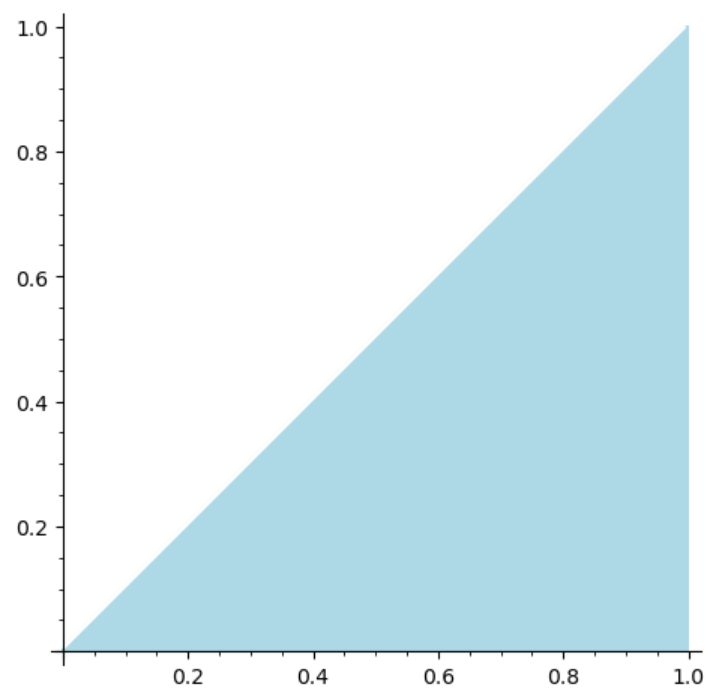
\includegraphics[width=0.7\linewidth]{images/5211}
	\caption{Miền $D: 0 \le x \le 1, \ 0 \le y \le x$}
	\label{fig:5211}
\end{figure}

\subsubsection{Toạ độ cực và tích phân trong toạ độ cực}
Xét tích phân:
\[ I = \iint\limits_D (x^2 + y^2) \, dx \, dy \quad \text{với } D \text{ là hình tròn tâm O bán kính 1}
\Rightarrow x = r\cos\theta, \ y = r\sin\theta \]
\begin{lstlisting}
	sage: var('r theta')
	sage: assume(r >= 0)
	sage: integrand = (r^2) * r  # x^2 + y^2 = r^2 va Jacobian la r
	sage: integrate(integrate(integrand, r, 0, 1), theta, 0, 2*pi)
	1/2*pi		# Ket qua
	sage: # Ve mien D
	sage: circle = implicit_plot(x^2 + y^2 == 1, (x, -1.2, 1.2), (y, -1.2, 1.2), color='red')
	sage: region = region_plot(lambda x, y: x^2 + y^2 <= 1, (x, -1, 1), (y, -1, 1), incol='lightgreen')
	show(region + circle)
\end{lstlisting}
\begin{figure}[H]
	\centering
	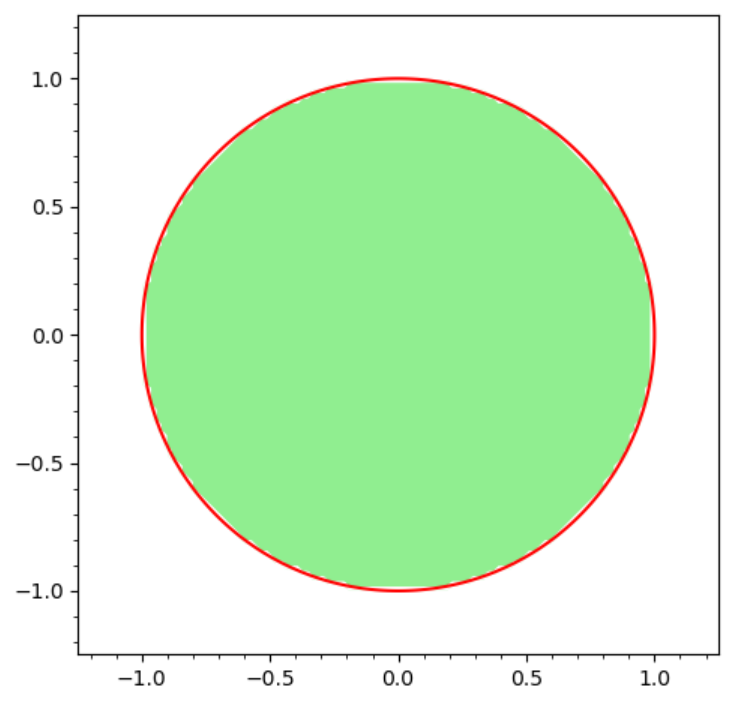
\includegraphics[width=0.7\linewidth]{images/5212}
	\caption{Miền D được vẽ bằng phương pháp tọa độ cực}
	\label{fig:5212}
\end{figure}

\subsubsection{Tích phân bội ba}
\[ I = \iiint\limits_E z \, dV \quad \text{với } E = \{(x, y, z) \mid 0 \le x \le 1, 0 \le y \le 1 - x, 0 \le z \le x + y \} \]
\begin{lstlisting}
	sage: var('x y z')
	sage: integrate(integrate(integrate(z, z, 0, x + y), y, 0, 1 - x), x, 0, 1)
	1/8		# Ket qua
\end{lstlisting}
\begin{figure}[H]
	\centering
	\begin{tikzpicture}
		\begin{axis}[axis lines=middle, xlabel={$x$}, ylabel={$y$}, zlabel={$z$},
			xmin=0, xmax=1, ymin=0, ymax=1, zmin=0, zmax=2,
			domain=0:1, view={30}{30}, width=8cm]
			
			\addplot3[surf, shader=interp] 
			{x + y};
			\addplot3[opacity=0.5, fill=blue] 
			{x*(1-x)};
		\end{axis}
	\end{tikzpicture}
	\caption{Mô phỏng miền tính tích phân bội ba}
	\label{fig:truc-toa-do}
\end{figure}

\subsection{Ứng dụng tích phân bội: diện tích, thể tích}
\subsubsection{Tính diện tích mặt phẳng}
\[ A = \iint\limits_D 1 \, dx \, dy \quad \text{với } D: 0 \le x \le 1, \ 0 \le y \le \sqrt{1 - x^2} \]
\begin{lstlisting}
	sage: integrate(integrate(1, y, 0, sqrt(1 - x^2)), x, 0, 1)
	1/4*pi		# Ket qua
	sage: # Ve mien D
	sage: f(x) = sqrt(1 - x^2)
	sage: p1 = plot(f(x), (x, 0, 1), fill=True, color='lightblue', legend_label="Vung D")
	sage: p1.show()
\end{lstlisting}
\begin{figure}[H]
	\centering
	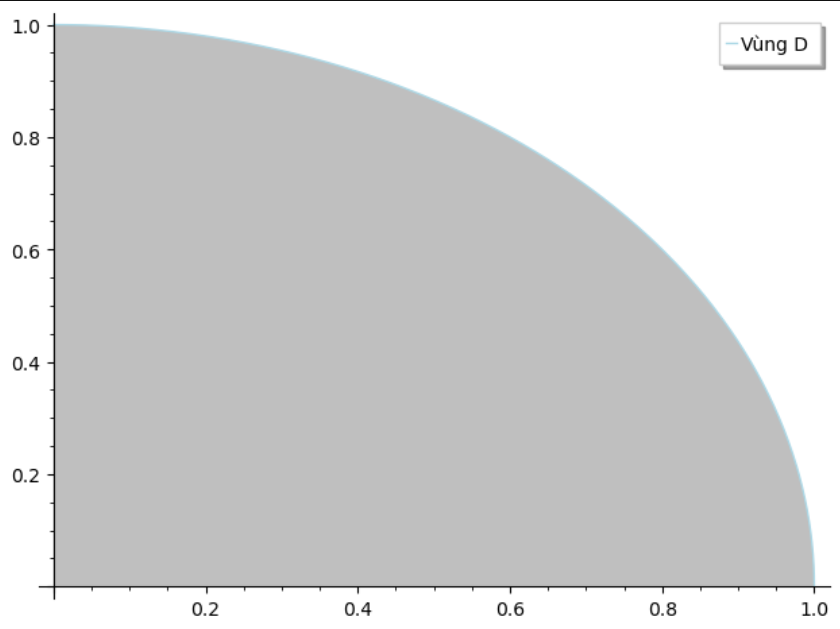
\includegraphics[width=0.7\linewidth]{images/5221}
	\caption{Miền cần tính diện tích $D: 0 \le x \le 1, \ 0 \le y \le \sqrt{1 - x^2}$}
	\label{fig:5221}
\end{figure}

\subsubsection{Thể tích vật thể}
Thể tích vật thể giới hạn bởi mặt phẳng \( z = x^2 + y^2 \) phía dưới và mặt phẳng \( z = 4 \) phía trên:
\begin{lstlisting}
	sage: var('r theta')
	sage: assume(r >= 0)
	sage: integrand = (4 - r^2) * r  # The tich = \int (z tren - z duoi)*Jacobian
	sage: integrate(integrate(integrand, r, 0, 2), theta, 0, 2*pi)
	8*pi 		# Ket qua 
\end{lstlisting}
\begin{figure}[ht!]
	\centering
	\begin{tikzpicture}
		\begin{axis}[
			axis lines = middle,
			view={30}{30},
			colormap/cool,
			enlargelimits,
			grid=both,
			]
			% Vẽ mặt phẳng z = x^2 + y^2 (phía dưới)
			\addplot3[
			domain=-2:2,
			y domain=-2:2,
			samples=50,
			samples y=50,
			z buffer=sort,
			surf,
			opacity=0.5,
			]
			{x^2 + y^2};
			
			% Vẽ mặt phẳng z = 4 (phía trên)
			\addplot3[
			domain=-2:2,
			y domain=-2:2,
			samples=50,
			samples y=50,
			z buffer=sort,
			surf,
			opacity=0.5,
			]
			{4};
		\end{axis}
	\end{tikzpicture}
	\caption{Mô phỏng miền vật thể giới hạn bởi mặt phẳng \( z = x^2 + y^2 \) phía dưới và mặt phẳng \( z = 4 \) phía trên.}
\end{figure}

\subsubsection{Tích phân phụ thuộc tham số}
\[ I(a) = \int_0^1 \frac{x^a - 1}{\ln x} \, dx \quad (a > 0) \]
\begin{lstlisting}
	sage: var('a x')
	sage: assume(a > 0)
	sage: integral = integrate((x^a - 1)/log(x), x, 0, 1)
	sage: integral
	I*pi + log(a + 1)
\end{lstlisting}

\subsection{Tích phân đường}
\subsubsection{Tích phân đường loại 1}
Tính \( \int_C f(x,y) ds \), với \( C: y = x^2, 0 \le x \le 1 \)
\begin{lstlisting}
	sage: f(x, y) = x + y
	sage: dx = 1
	sage: dy = diff(x^2, x)
	sage: ds = sqrt(dx^2 + dy^2)
	sage: I = integrate(f(x, x^2)*ds, x, 0, 1)
	sage: I
	67/96*sqrt(5) - 1/64*arcsinh(2) - 1/12		#Ket qua
	sage: # Ve mien D
	sage: var('x y')
	sage: f(x) = x^2
	sage: plot1 = plot(f(x), (x, 0, 1), color='blue', sage: legend_label='y = x^2')
	sage: f_xy(x, y) = x + y
	sage: plot1.show()
	
\end{lstlisting}
\begin{figure}[H]
	\centering
	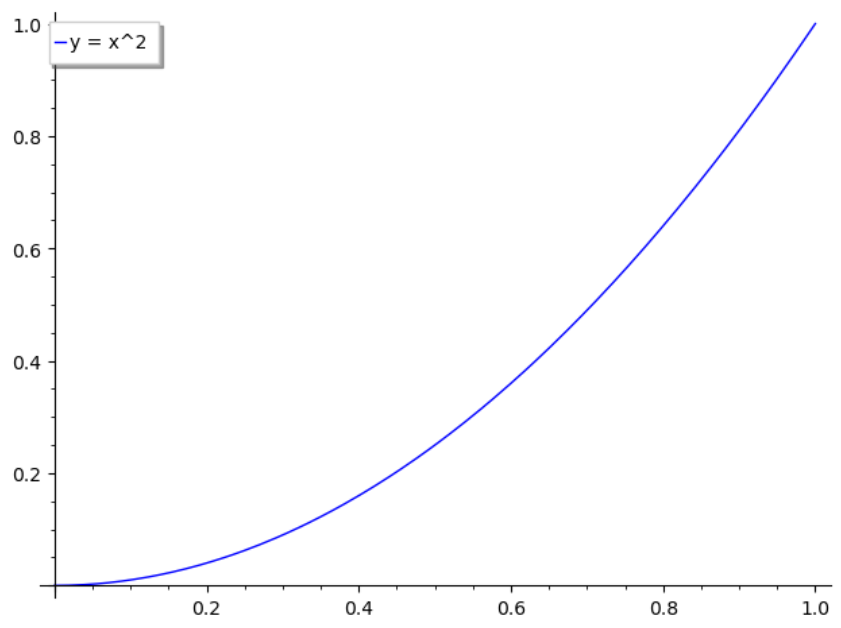
\includegraphics[width=0.5\linewidth]{images/5231}
	\caption{Miền $C: y = x^2, 0 \le x \le 1$}
	\label{fig:5231}
\end{figure}


\subsubsection{Tích phân đường loại 2}
Tính \( \int_C (x \, dx + y \, dy) \), với \( C \) là đường tròn đơn vị.
\begin{lstlisting}
	sage: x(t) = cos(t)
	sage: y(t) = sin(t)
	sage: dx = diff(x(t), t)
	sage: dy = diff(y(t), t)
	sage: integrand = x(t)*dx + y(t)*dy
	sage: integrate(integrand, t, 0, 2*pi)
	0		# Ket qua
	sage: # Ve mien D
	sage: var('t')
	sage: x(t) = cos(t)
	sage: y(t) = sin(t)
	sage: parametric_plot((x(t), y(t)), (t, 0, 2*pi), color='blue', legend_label='C: x(t), y(t)')
\end{lstlisting}
\begin{figure}[H]
	\centering
	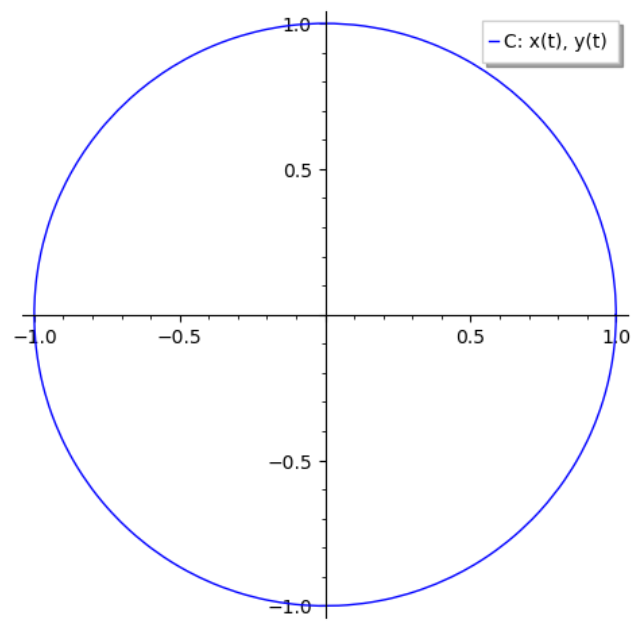
\includegraphics[width=0.5\linewidth]{images/5232}
	\caption{Miền $C$ là đường tròn đơn vị}
	\label{fig:5232}
\end{figure}


\subsection{Tích phân mặt}
Tính tích phân mặt của hàm \( f(x, y, z) = z \) trên mặt phẳng \( z = 1 - x - y, 0 \le x, y \le 1, x + y \le 1 \)
\begin{lstlisting}
	sage: z(x, y) = 1 - x - y
	sage: f(x, y) = z(x, y)
	sage: I = integrate(integrate(f(x, y), y, 0, 1 - x), x, 0, 1)
	sage: I
	1/6		# Ket qua
\end{lstlisting}
\begin{figure}[H]
	\centering
	\tdplotsetmaincoords{70}{120}
	\begin{tikzpicture}[tdplot_main_coords, scale=5]
		
		% Trục tọa độ
		\draw[->] (0,0,0) -- (1.1,0,0) node[anchor=north east]{$x$};
		\draw[->] (0,0,0) -- (0,1.1,0) node[anchor=north west]{$y$};
		\draw[->] (0,0,0) -- (0,0,1.1) node[anchor=south]{$z$};
		
		% Các điểm tam giác
		\coordinate (A) at (1,0,0);
		\coordinate (B) at (0,1,0);
		\coordinate (C) at (0,0,1);
		
		% Mặt phẳng z = 1 - x - y là tam giác ABC
		\filldraw[fill=blue!30, opacity=0.7] (A) -- (B) -- (C) -- cycle;
		
		% Nhãn điểm
		\node at (A) [below right] {$(1,0,0)$};
		\node at (B) [above left] {$(0,1,0)$};
		\node at (C) [above right] {$(0,0,1)$};
		
	\end{tikzpicture}
	\caption{Mặt phẳng $z = 1 - x - y$ trên miền tam giác $x + y \leq 1$}
\end{figure}

\subsection{Lý thuyết trường}
\subsubsection{Đạo hàm theo hướng}
Tính đạo hàm theo hướng của \( f(x, y) = x^2y \) tại \( A(1, 2) \) theo hướng \( \vec{v} = (3, 4) \)
\begin{lstlisting}
	sage: f(x, y) = x^2*y
	sage: u = vector([3, 4]).normalized()
	sage: grad_f = vector([diff(f(x, y), x), diff(f(x, y), y)])
	sage: point = vector([1, 2])
	sage: grad_at_A = grad_f.subs(x=point[0], y=point[1])
	sage: directional_derivative = grad_at_A.dot_product(u)
	sage: directional_derivative
	16/5	# Ket qua
	
	sage: # Ve mien D
	sage: var('x y')
	sage: # Ham so
	sage: f(x, y) = x^2 * y
	sage: # Diem A
	sage: A = vector([1, 2])
	sage: # Vector huong
	sage: v = vector([3, 4])
	sage: u = v.normalized()
	sage: # Gradient
	sage: grad_f = vector([diff(f(x, y), x), diff(f(x, y), y)])
	sage: grad_A = grad_f.subs(x=A[0], y=A[1])
	sage: # Vector dao ham theo huong
	sage: D_u_f = grad_A.dot_product(u)
	sage: vec_D = D_u_f * u
	sage: # Ve mat ham
	sage: surface = plot3d(f(x, y), (x, 0, 2), (y, 0, sage: 2), opacity=0.6, color='lightblue')
	sage: # Ve diem A tren mat
	sage: pointA = point3d((A[0], A[1], f(*A)), color='red', size=30)
	sage: # Ve gradient tai A
	sage: grad_arrow = arrow3d((A[0], A[1], f(*A)), (A[0] + grad_A[0], A[1] + grad_A[1], f(*A)), color='green', width=2)
	sage: # Ve vector huong tai A
	sage: u_arrow = arrow3d((A[0], A[1], f(*A)), (A[0] + u[0], A[1] + u[1], f(*A)), color='orange', width=2)
	sage: # Ve vector dao ham theo huong (chi phan vector tren mat, khong tang do cao)
	sage: vecD_arrow = arrow3d((A[0], A[1], f(*A)), (A[0] + vec_D[0], A[1] + vec_D[1], f(*A)), color='purple', width=2)
	sage: # Gop cac thanh phan
	sage: show(surface + pointA + grad_arrow + u_arrow + vecD_arrow, frame=True)
	
\end{lstlisting}
\begin{figure}[H]
	\centering
	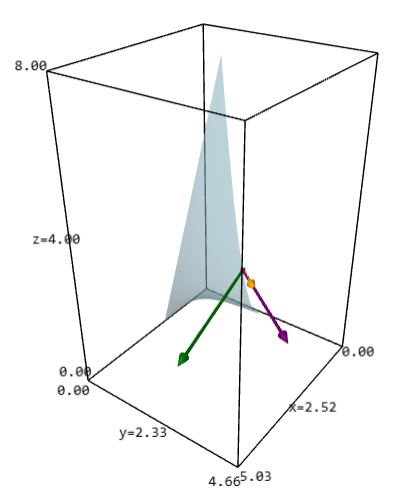
\includegraphics[width=0.7\linewidth]{images/5251}
	\caption{Đồ thị mô phỏng đạo hàm theo hướng của \( f(x, y) = x^2y \) tại \( A(1, 2) \) theo hướng \( \vec{v} = (3, 4) \)}
	\label{fig:5251}
\end{figure}

\subsubsection{Tính gradient}
\begin{lstlisting}
	sage: var('x y')
	sage: f(x, y) = x^2 * y
	sage: # Tinh gradient thu cong
	sage: grad_f = vector([diff(f(x, y), x), diff(f(x, y), y)])
	sage: grad_f
	(2*x*y, x^2)
\end{lstlisting}

\newpage
\section{Ứng dụng trong Giải tích 3}

\subsection{Chuỗi số, xét sự hội tụ của chuỗi số}
Xét sự hội tụ của chuỗi: $\sum_{n=1}^{\infty} \dfrac{1}{n^p}$ với $p>1$.
\begin{lstlisting}
	sage: var('n')
	sage: f = 1/n^100
	sage: sum(f, n, 1, oo)
	sage: var('n')
	sage: f = 1/n^100
	sage: sum(f, n, 1, oo)
	189196075638244.../981520542075751...*pi^100	# Ket qua +oo
\end{lstlisting}

\subsection{Chuỗi hàm, tính tổng chuỗi, chuỗi hội tụ đều}
Tính tổng chuỗi hàm $\sum_{n=0}^{\infty}{\dfrac{x^n}{n!}}$
\begin{lstlisting}
	sage: var('x n')
	sage: f = x^n/factorial(n)
	sage: S = sum(f, n, 0, oo)
	sage: S
	e^x			# Ket qua
\end{lstlisting}

\subsection{Chuỗi lũy thừa, khai triển Taylor, Maclaurin}
Khai triển chuỗi Maclaurin của $\sin{x}$.
\begin{lstlisting}
	sage: taylor(sin(x), x, 0, 7)
	-1/5040*x^7 + 1/120*x^5 - 1/6*x^3 + x		# Ket qua
\end{lstlisting}

\subsection{Chuỗi Fourier, khai triển Fourier}
Khai triển chuỗi Fourier của $f(x)=x$ trên $\left[-\pi,\pi\right]$.
\begin{lstlisting}
	sage: var('x n')
	sage: f(x) = x
	sage: a0 = (1/pi)*integrate(f(x), x, -pi, pi)
	sage: a0
	0
	sage: an = (1/pi)*integrate(f(x)*cos(n*x), x, -pi, pi)
	sage: an
	0
	sage: bn = (1/pi)*integrate(f(x)*sin(n*x), x, -pi, pi)
	sage: bn
	-2*(pi*n*cos(pi*n) - sin(pi*n))/(pi*n^2)

	# Ve do thi khai trien Fourier bac 5
	sage: fourier = sum(2*(-1)^(k+1)/k*sin(k*x) for k in (1..5))
	sage: p1 = plot(f(x), (x, -pi, pi), color='blue', legend_label='f(x)=x')
	sage: p2 = plot(fourier, (x, -pi, pi), color='red', legend_label='Fourier')
	sage: show(p1 + p2)
\end{lstlisting}
\begin{figure}[H]
	\centering
	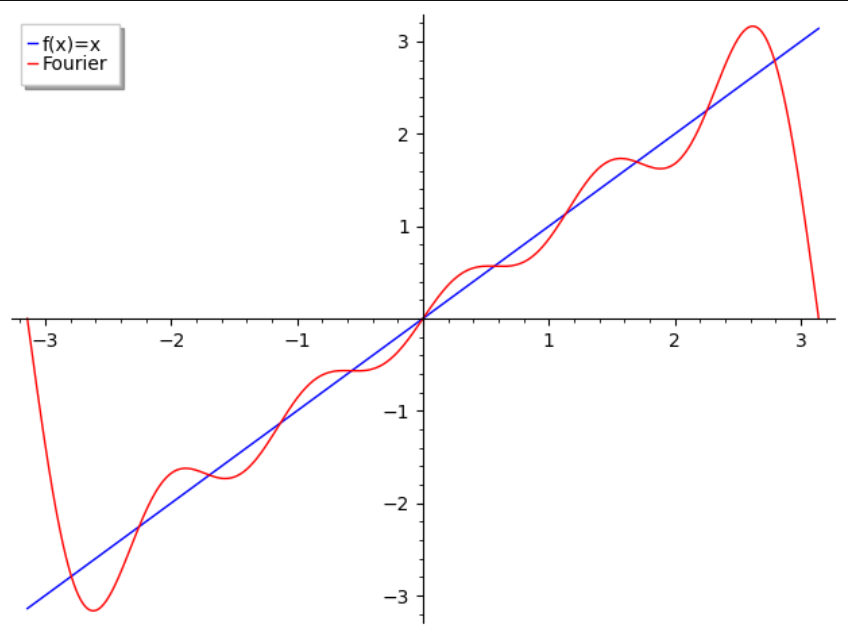
\includegraphics[width=0.7\linewidth]{images/534}
	\caption{Đồ thị minh họa khai triển chuỗi Fourier của $f(x)=x$ trên $\left[-\pi,\pi\right]$}
	\label{fig:534}
\end{figure}


\subsection{Giải phương trình vi phân tuyến tính cấp 1, cấp 2}
Giải phương trình:
\[
y' + y = e^x
\]
\begin{lstlisting}
	sage: var('x y')
	sage: y = function('y')(x)
	sage: de = diff(y, x) + y == e^x
	sage: desolve(de, y)
	1/2*(2*_C + e^(2*x))*e^(-x)		# Ket qua
\end{lstlisting}
Giải phương trình:
\[
y'' - y = 0
\]	
\begin{lstlisting}
	sage: y = function('y')(x)
	sage: de2 = diff(y, x, 2) - y == 0
	sage: desolve(de2, y)
	_K2*e^(-x) + _K1*e^x		# Ket qua
\end{lstlisting}

\subsection{Giải phương trình Euler}
Giải phương trình vi phân Euler:
\[
x^2 y'' - x y' + y = 0
\]
\begin{lstlisting}
	sage: y = function('y')(x)
	sage: de = x^2*diff(y, x, 2) - x*diff(y, x) + y == 0
	sage: desolve(de, y)
	(_K2*log(x) + _K1)*x		# Ket qua
\end{lstlisting}

\subsection{Giải hệ phương trình vi phân cấp 1}
Giải hệ:
\[
\begin{cases}
	x' = x + y \\
	y' = x - y
\end{cases}
\]
\begin{lstlisting}
	sage: t = var('t')
	sage: x = function('x')(t)
	sage: y = function('y')(t)
	sage: de1 = diff(x, t) == x + y
	sage: de2 = diff(y, t) == x - y
	sage: desolve_system([de1, de2], [x, y])
	[x(t) == 1/2*sqrt(2)*(x(0) + y(0))*sinh(sqrt(2)*t) + cosh(sqrt(2)*t)*x(0),
	y(t) == 1/2*sqrt(2)*(x(0) - y(0))*sinh(sqrt(2)*t) + cosh(sqrt(2)*t)*y(0)]
\end{lstlisting}

\subsection{Biến đổi Laplace, ứng dụng giải phương trình vi phân}
Giải phương trình bằng biến đổi Laplace:
\[
y'' + y = \sin(t), \quad y(0) = 0,\ y'(0) = 1
\] 
\begin{lstlisting}
	sage: var('t s')
	sage: y = function('y')(t)
	sage: de = diff(y, t, 2) + y == sin(t)
	sage: desolve_laplace(de, y, ivar=t)
	-1/2*t*cos(t) + 1/2*(2*D[0](y)(0) + 1)*sin(t) + cos(t)*y(0)		# Ket qua
\end{lstlisting}

\section{Ứng dụng trong Đại số tuyến tính}

\subsection{Các phép toán Logic, tập hợp}
Các phép toán logic và phép toán trên tập hợp có thể được thực hiện bằng các công cụ trong SageMath. Ví dụ, để tính toán hợp, giao, hiệu của các tập hợp, hoặc thực hiện các phép toán logic như AND, OR, NOT, ta có thể sử dụng cú pháp sau.

\begin{lstlisting}
	sage: # Hop va giao cua tap hop
	sage: A = Set([1, 2, 3])
	sage: B = Set([3, 4, 5])
	sage: A.union(B)  # Hop
	{1, 2, 3, 4, 5}
	sage: A.intersection(B)  # Giao
	{3}
\end{lstlisting}

\subsection{Ánh xạ, tìm ảnh và nghịch ảnh}
Để tính ảnh và nghịch ảnh trong ánh xạ, ta có thể áp dụng trực tiếp công thức của ánh xạ. Ví dụ dưới đây minh họa cách tìm ảnh và nghịch ảnh của một số trong ánh xạ \( f(x) = x^2 \).

\begin{lstlisting}
	sage: var('x')
	sage: f = x^2
	sage: f(x=3)  # Tinh anh cua 3
	9
	sage: f.inverse_function()(9)  # Tim nghich anh cua 9
\end{lstlisting}

\subsection{Cấu trúc đại số nhóm, vành, trường, nhóm Abel}
Các phép toán trong các cấu trúc đại số như nhóm, vành và trường có thể thực hiện thông qua các phép toán trong SageMath. Các phép toán nhóm Abel có thể sử dụng phép toán nhóm trong Sage.

\begin{lstlisting}
	# Phep toan nhom Abel
	G = Group([(1, 1), (2, 2)])
	G * G  # Nhan nhom
\end{lstlisting}

\subsection{Số phức, tính module, phép toán số phức, thu gọn về dạng chính tắc}
Các phép toán với số phức như cộng, trừ, nhân, chia, tính module và thu gọn về dạng chính tắc có thể thực hiện trong SageMath. Dưới đây là cách tính module và thu gọn số phức về dạng chính tắc.

\begin{lstlisting}
	sage: z = 3 + 4*I  # So phuc
	sage: abs(z)  # Tinh module
	5
	sage: conjugate(z)  # Tinh phan ao
	11/3
\end{lstlisting}

\subsection{Tìm căn bậc n của số phức, giải phương trình nghiệm phức}
Để tìm căn bậc n của số phức hoặc giải phương trình nghiệm phức, ta sử dụng các hàm \texttt{nth\_root} và \texttt{solve}.

\begin{lstlisting}
	sage: z = 1 + I
	sage: nth_root(z, 3)  # Tim can bac 3 cua z
	sage: solve(x^2 + 1 == 0, x)  # Giai phuong trinh x^2 + 1 = 0
\end{lstlisting}

\subsection{Ma trận và các phép toán ma trận, định thức, ma trận nghịch đảo, ma trận mũ, hạng của ma trận, hệ phương trình tuyến tính (Phương pháp Gauss)}
Các phép toán ma trận như tính định thức, nghịch đảo, ma trận mũ và hạng có thể thực hiện dễ dàng trong SageMath. Hệ phương trình tuyến tính có thể giải bằng phương pháp Gauss.

\begin{lstlisting}
	sage: A = Matrix([[1, 2], [3, 4]])
	sage: det(A)  # Tinh dinh thuc
	sage: A.inv()  # Tinh ma tran nghich dao
	sage: A^2  # Ma tran mu
	sage: A.rank()  # Hang cua ma tran
	sage: solve(A*x == [1, 2], x)  # Giai he phuong trinh tuyen tinh
\end{lstlisting}

\subsection{Không gian vector, kiểm tra hệ độc lập tuyến tính}
Để kiểm tra tính độc lập tuyến tính của các vector, ta có thể tính hạng của ma trận tạo thành từ các vector đó.

\begin{lstlisting}
	sage: v1 = vector([1, 2])
	sage: v2 = vector([2, 4])
	sage: matrix([v1, v2]).rank()  # Kiem tra tinh doc lap tuyen tinh
\end{lstlisting}

\subsection{Tìm cơ sở và số chiều sinh bởi hệ vector}
Cơ sở của không gian vector có thể tìm được thông qua phép biến đổi ma trận, ví dụ dưới đây minh họa cách tìm cơ sở và số chiều sinh bởi hệ vector.

\begin{lstlisting}
	sage: v1 = vector([1, 0])
	sage: v2 = vector([0, 1])
	sage: matrix([v1, v2]).column_space()  # Tim co so
\end{lstlisting}

\subsection{Ánh xạ tuyến tính, giá trị riêng và vector riêng}
Các phép toán như tìm giá trị riêng và vector riêng của một ma trận có thể được thực hiện qua hàm `eigenvalues` và `eigenvectors`.

\begin{lstlisting}
	sage: A = Matrix([[1, 2], [3, 4]])
	sage: A.eigenvalues()  # Tinh gia tri rieng
	sage: A.eigenvectors()  # Tinh vector rieng
\end{lstlisting}

\subsection{Chéo hóa ma trận}
Chéo hóa ma trận có thể thực hiện bằng cách sử dụng hàm `diagonalize`, nếu ma trận có đủ số lượng vector riêng độc lập.

\begin{lstlisting}
	sage: A = Matrix([[4, 1], [2, 3]])
	sage: A.diagonalize()  # Cheo hoa ma tran
\end{lstlisting}

\subsection{Trực chuẩn hóa cơ sở, xác định ma trận chuyển cơ sở, tìm hình chiếu trực giao}
Các phép toán như chuẩn hóa cơ sở, ma trận chuyển cơ sở và hình chiếu trực giao có thể thực hiện bằng các phép toán ma trận và vector trong SageMath.

\begin{lstlisting}
	sage: v1 = vector([1, 0])
	sage: v2 = vector([0, 1])
	sage: v1.normalized()  # Chuan hoa vector
	sage: projection = v1.project_onto(v2)  # Tinh hinh chieu truc giao
\end{lstlisting}

\subsection{Vẽ các đường cong phẳng, mặt bậc hai}
Để vẽ các đường cong phẳng và mặt bậc hai, ta có thể sử dụng các hàm vẽ 2D và 3D trong SageMath. Dưới đây là cách vẽ đường cong và mặt bậc hai.

\begin{lstlisting}
	sage: plot(x^2 + y^2, (x, -2, 2), (y, -2, 2))  # Ve duong cong
	sage: implicit_plot3d(x^2 + y^2 - z, (x, -2, 2), (y, -2, 2), (z, 0, 10))  # Ve mat bac hai
\end{lstlisting}

\section{Ứng dụng trong Xác suất thống kê}

\subsection{Tổ hợp, chỉnh hợp, giai thừa}
SageMath hỗ trợ các hàm tính tổ hợp và giai thừa để giải các bài toán xác suất. Tuy nhiên, SageMath không có sẵn hàm tính chỉnh hợp, nên ta sẽ sử dụng cách tính theo đúng công thức $P(n,k)=\dfrac{n!}{(n-k)!}$.

\begin{lstlisting}
	# Tinh giai thua
	sage: factorial(5)
	120
	
	# Tinh to hop chap 3 cua 5
	sage: binomial(5, 3)
	10
	
	# Tinh chinh hop chap 2 cua 4
	sage: factorial(4) / factorial(4 - 2)
	12
\end{lstlisting}

\subsection{Biến ngẫu nhiên và phân phối xác suất}
SageMath có các hàm tích hợp để tính kỳ vọng, phương sai và độ lệch chuẩn của các biến ngẫu nhiên.

\begin{lstlisting}
	# Tinh ky vong va phuong sai cua bien ngau nhien
	sage: var('x p')
	sage: X = [1, 2, 3]
	sage: P = [0.2, 0.5, 0.3]
	sage: mean = sum(x * p for x, p in zip(X, P))
	sage: variance = sum((x - mean)^2 * p for x, p in zip(X, P))
	sage: mean, variance
	(2.10000000000000, 0.490000000000000)
\end{lstlisting}

Ta cũng có thể sử dụng từ thư viện \texttt{NumPy} để tính giá trị trung bình (mean), phương sai (variance) và độ lệch chuẩn như sau:
\begin{lstlisting}
	# Tinh ky vong va phuong sai cua bien ngau nhien voi NumPy
	sage: import numpy as np
	sage: data = [10, 20, 30, 40, 50]
	sage: mean = np.mean(data)
	sage: variance = np.var(data)
	sage: std_dev = np.std(data)
	sage: mean, variance, std_dev
	(30.0, 200.0, 14.142135623730951)
\end{lstlisting}
Hoặc sử dụng hàm từ \texttt{SciPy}:
\begin{lstlisting}
	# Tinh ky vong va phuong sai cua bien ngau nhien voi SciPy
	sage: from scipy.stats import describe
	sage: data = [10, 20, 30, 40, 50]
	sage: stats = describe(data)
	sage: stats.mean, stats.variance
	(30.0, 200.0)
\end{lstlisting}

\subsubsection{Vẽ đồ thị phân phối xác suất}
Dưới đây là ví dụ vẽ đồ thị phân phối nhị thức với SageMath.

\begin{lstlisting}
	# Ve do thi phan phoi nhi thuc voi p = 0.5, n = 10
	sage: var('k')
	sage: p = 0.5
	sage: n = 10
	sage: P = [binomial(n, k) * p^k * (1 - p)^(n - k) for k in range(n + 1)]
	sage: bar_chart(P, width=0.5, title='Phan phoi nhi thuc', axes=True)
\end{lstlisting}
\begin{figure}[H]
	\centering
	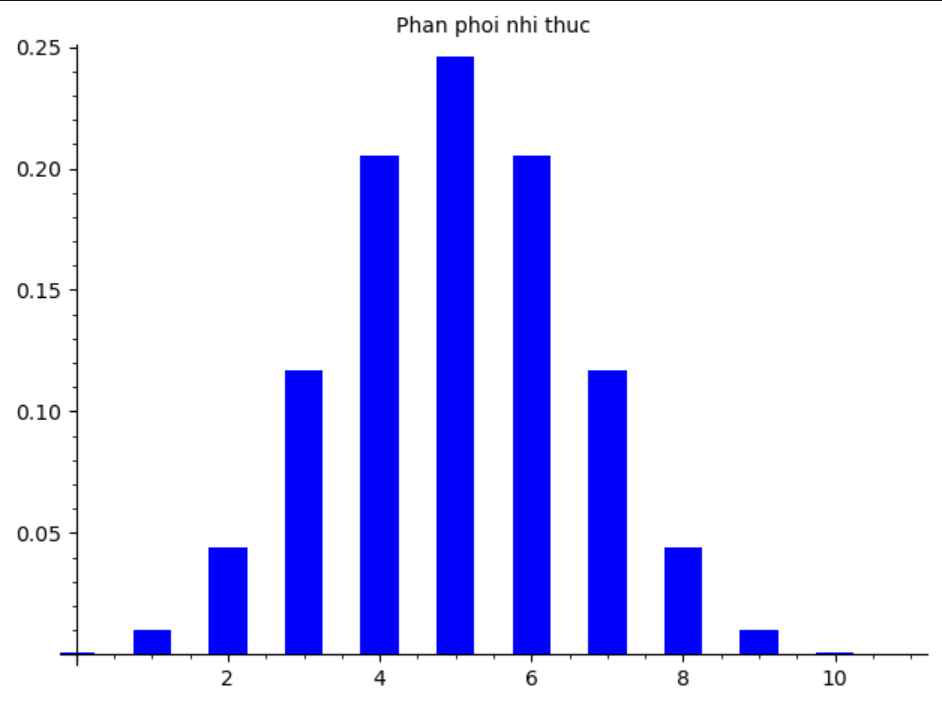
\includegraphics[width=0.7\linewidth]{images/screenshot001}
	\caption{Biểu đồ phân phối nhị thức với $(n,p)=(10,0.5)$}
	\label{fig:screenshot001}
\end{figure}

\subsection{Biến ngẫu nhiên nhiều chiều}
Tính hàm mật độ xác suất biên và xác suất điều kiện.

\begin{lstlisting}
	# Phan phoi xac suat bien
	sage: var('x y')
	sage: f = x * y
	sage: integrate(f, (x, 0, 1))  # Ham mat do xac suat bien theo y
	1/2 * y^2
\end{lstlisting}

\subsection{Ước lượng tham số}
Tính khoảng tin cậy cho kỳ vọng và tỷ lệ.

\begin{lstlisting}
	# Uoc luong ky vong voi do tin cay 95%
	sage: var('x n s')
	sage: mu = x + 1.96 * s / sqrt(n)
	sage: mu.subs({x: 50, s: 10, n: 100})
	51.9600000000000
\end{lstlisting}

\subsection{Kiểm định giả thuyết}
Thực hiện kiểm định giả thuyết với mẫu và tính p-value.

\begin{lstlisting}
	# Kiem dinh Z
	sage: var('xbar mu sigma n')
	sage: Z = (xbar - mu) / (sigma / sqrt(n))
	sage: Z.subs({xbar: 110, mu: 100, sigma: 15, n: 30})
	3.651483716701107
\end{lstlisting}

\subsection{Thống kê mô tả và suy diễn}
Tính các tham số thống kê như trung bình, phương sai, độ lệch chuẩn.

\begin{lstlisting}
	# Thong ke mo ta voi scipy
	sage: from scipy.stats import describe
	sage: data = [10, 20, 30, 40, 50]
	sage: describe(data)
	# Ket qua: N, min, max, mean, variance
	DescribeResult(nobs=5, minmax=(10, 50), mean=30.0, variance=250.0, skewness=0.0, kurtosis=-1.3)
\end{lstlisting}

\subsection{Phân tích hồi quy}
Hồi quy tuyến tính và kiểm định độ phù hợp của mô hình.

\begin{lstlisting}
	# Hoi quy tuyen tinh
	sage: var('x')
	sage: data = [(1, 2), (2, 4), (3, 6)]
	sage: m, b = var('m b')
	sage: model = m * x + b
	sage: eqs = [model.subs(x=xv) == yv for xv, yv in data]
	sage: solve(eqs, m, b)
	[[m == 2, b == 0]]
\end{lstlisting}

\subsection{Phân tích phương sai (ANOVA)}
Phân tích phương sai để kiểm định giả thuyết về nhiều trung bình.

\begin{lstlisting}
	# Phan tich ANOVA
	sage: from scipy.stats import f_oneway
	sage: group1 = [23, 20, 25, 22]
	sage: group2 = [27, 29, 30, 28]
	sage: f_oneway(group1, group2)
	# Ket qua: p-value va thong ke F
	F_onewayResult(statistic=24.0, pvalue=0.002713682035093796)
\end{lstlisting}

	
	% Chương 7: Kết luận và hướng phát triển
	\chapter{Kết luận và hướng phát triển}
	\section{Tổng kết nội dung nghiên cứu}

Trong quá trình thực hiện đồ án, em đã nghiên cứu và triển khai việc sử dụng SageMath vào giải quyết các bài toán toán học thuộc nhiều môn học khác nhau trong các học phần Toán đại cương tại Đại học Bách Khoa Hà Nội. 

Thông qua việc khai thác các tính năng cốt lõi của SageMath, em đã đạt được những kết quả đáng khích lệ như sau:
\begin{itemize}
	\item Tìm hiểu và ứng dụng các phép toán cơ bản và nâng cao trong SageMath, bao gồm tính toán đại số, giải tích, tổ hợp, thống kê và các phép toán số học.
	\item Sử dụng các hàm hỗ trợ mạnh mẽ của SageMath để giải quyết các bài toán thực tiễn như tính giới hạn, tích phân, đạo hàm, giải hệ phương trình tuyến tính, chéo hóa ma trận và phân tích Fourier.
	\item Xây dựng các ứng dụng tính toán thực tiễn trong các học phần Toán đại cương, từ các bài toán đại số trừu tượng đến các phép tính trong giải tích số và toán rời rạc.
	\item Tạo các đồ thị trực quan, minh họa các khái niệm toán học thông qua các hàm vẽ đồ thị 2D, 3D, biểu đồ phân phối xác suất, biểu đồ hàm số và các hình học không gian.
	\item Thiết kế SageMath Notebook giúp thầy cô và các bạn sinh viên tương tác và kiểm tra trực tiếp các ví dụ, bài tập, đồng thời tích hợp các thư viện Python để mở rộng khả năng tính toán.
\end{itemize}

Kết quả của đồ án đã chứng minh rằng SageMath là một công cụ mạnh mẽ trong việc hỗ trợ giảng dạy và nghiên cứu toán học, đặc biệt là trong các học phần Toán đại cương tại các trường đại học. Việc tích hợp SageMath vào quá trình học tập giúp sinh viên rèn luyện kỹ năng tính toán, tư duy lập trình, cũng như khả năng phân tích và trực quan hóa dữ liệu toán học.

Tuy nhiên, trong quá trình thực hiện, em cũng nhận thấy một số hạn chế cần khắc phục, sẽ được trình bày trong các phần tiếp theo. Bên cạnh đó, đồ án cũng mở ra những hướng nghiên cứu mới nhằm cải thiện việc ứng dụng SageMath trong giáo dục và nghiên cứu khoa học.

\section{Những khó khăn và hạn chế của SageMath}

Trong quá trình tìm hiểu và sử dụng SageMath, em đã gặp phải một số khó khăn và hạn chế, cả về mặt kỹ thuật lẫn trong việc ứng dụng vào các bài toán thực tiễn. Dưới đây là một số vấn đề nổi bật mà em nhận thấy:

\subsection{Khó khăn trong cài đặt và cấu hình}

Việc cài đặt SageMath không phải lúc nào cũng đơn giản, đặc biệt trên các hệ điều hành như Windows. Một số khó khăn em gặp phải bao gồm:
\begin{itemize}
	\item SageMath yêu cầu dung lượng lớn và tài nguyên hệ thống tương đối cao.
	\item Việc tích hợp với các công cụ như Jupyter Notebook đôi khi gặp lỗi phiên bản và xung đột thư viện.
	\item Cài đặt SageMath trên Windows thường đòi hỏi sử dụng WSL (Windows Subsystem for Linux), gây khó khăn cho những người không quen với môi trường Linux.
\end{itemize}

\subsection{Hạn chế về khả năng tính toán và thư viện}

Mặc dù SageMath tích hợp nhiều thư viện mạnh mẽ, nhưng trong một số trường hợp đặc biệt, em nhận thấy có những hạn chế như sau:
\begin{itemize}
	\item Một số phép toán phức tạp như tính giới hạn, tích phân đa biến hoặc giải phương trình vi phân đôi khi không cho kết quả chính xác hoặc không hỗ trợ trực tiếp.
	\item Các hàm thống kê và phân phối xác suất chưa phong phú so với các phần mềm chuyên dụng như R hoặc MATLAB.
	\item Việc xử lý dữ liệu lớn đôi khi không hiệu quả do thiếu các hàm tối ưu hóa chuyên dụng.
\end{itemize}

\subsection{Hạn chế trong việc trực quan hóa}

Mặc dù SageMath hỗ trợ vẽ đồ thị 2D và 3D, nhưng khi so sánh với các phần mềm như Mathematica hay MATLAB, khả năng trực quan hóa còn hạn chế:
\begin{itemize}
	\item Việc tùy chỉnh đồ thị phức tạp đòi hỏi nhiều mã lệnh và không thân thiện với người mới bắt đầu.
	\item Các đồ thị 3D khi vẽ trong môi trường notebook có thể bị chậm và khó thao tác.
	\item Việc kết hợp nhiều đồ thị trên cùng một hệ trục không dễ dàng như trong các phần mềm chuyên nghiệp.
\end{itemize}

\subsection{Khó khăn trong việc học và sử dụng}

SageMath là một hệ thống mạnh mẽ nhưng không dễ tiếp cận đối với sinh viên mới làm quen với lập trình:
\begin{itemize}
	\item Cú pháp của SageMath đôi khi gây nhầm lẫn vì nó kết hợp nhiều thư viện từ các ngôn ngữ khác nhau.
	\item Tài liệu hướng dẫn chính thức chưa thật sự đầy đủ, đặc biệt đối với các chức năng nâng cao.
	\item Việc tìm kiếm giải pháp cho các lỗi gặp phải trong quá trình sử dụng cũng là một thách thức, do cộng đồng người dùng không lớn bằng các phần mềm thương mại.
\end{itemize}

\section{Định hướng phát triển và nghiên cứu trong tương lai}

Trong quá trình thực hiện đồ án, em nhận thấy SageMath là một công cụ mạnh mẽ nhưng vẫn còn nhiều tiềm năng chưa được khai thác hết. Để nâng cao hiệu quả sử dụng, em xin đề xuất một số định hướng phát triển trong tương lai như sau:

\subsection{Tích hợp AI để chuyển ngôn ngữ tự nhiên thành mã SageMath}

Một trong những khó khăn lớn nhất đối với người dùng SageMath là phải thành thạo cú pháp và các hàm toán học trong phần mềm. Điều này đòi hỏi thời gian học tập và nắm vững ngôn ngữ lập trình của SageMath. 

Để khắc phục vấn đề này, em đề xuất sử dụng trí tuệ nhân tạo (AI) để tự động chuyển đổi ngôn ngữ tự nhiên thành mã SageMath. Mô hình AI sẽ nhận đầu vào là câu lệnh toán học từ người dùng bằng ngôn ngữ tự nhiên, sau đó chuyển đổi thành mã SageMath, thực thi lệnh và trả về kết quả. Điều này sẽ giúp người dùng giải toán mà không cần học SageMath, nâng cao trải nghiệm sử dụng phần mềm, đặc biệt đối với sinh viên và người dùng không chuyên.

\subsection{Phát triển giao diện thân thiện người dùng}

Một trong những yếu tố quan trọng giúp SageMath tiếp cận rộng rãi hơn là việc cải thiện giao diện sử dụng. Hiện tại, giao diện của SageMath chủ yếu dựa trên dòng lệnh hoặc Jupyter Notebook, gây khó khăn cho người mới bắt đầu. 

Trong tương lai, cần phát triển một ứng dụng trực quan hơn, có giao diện đồ họa giống như các phần mềm thương mại khác như Mathematica hay MATLAB. Giao diện này sẽ hỗ trợ:
\begin{itemize}
	\item Nhập công thức toán học trực tiếp bằng cách kéo thả các biểu thức.
	\item Hiển thị kết quả ngay lập tức mà không cần chạy mã lệnh.
	\item Tích hợp các tính năng vẽ đồ thị, giải phương trình và biểu diễn ma trận với các nút bấm trực quan.
\end{itemize}

\subsection{Xây dựng thư viện bài tập và tài liệu hỗ trợ học tập}

Để hỗ trợ sinh viên trong quá trình học tập và nghiên cứu, em đề xuất xây dựng một thư viện bài tập và hướng dẫn giải chi tiết bằng SageMath. Thư viện này sẽ bao gồm:
\begin{itemize}
	\item Các bài tập từ cơ bản đến nâng cao thuộc các học phần Toán đại cương.
	\item Ví dụ minh họa và mã SageMath tương ứng để sinh viên dễ dàng tiếp cận.
	\item Tài liệu giải thích các tính năng quan trọng của SageMath kèm theo ví dụ thực hành.
\end{itemize}

\subsection{Tăng cường khả năng tính toán thống kê và xử lý dữ liệu lớn}

Mặc dù SageMath đã tích hợp các thư viện thống kê và tính toán số học như NumPy, SciPy, nhưng vẫn chưa đáp ứng được nhu cầu xử lý dữ liệu lớn và phân tích thống kê phức tạp. Trong tương lai, cần:
\begin{itemize}
	\item Tích hợp chặt chẽ hơn với các thư viện chuyên dụng như Pandas và R.
	\item Tối ưu hóa hiệu năng để tính toán nhanh hơn khi xử lý dữ liệu lớn.
	\item Cải thiện các hàm thống kê và phân tích dữ liệu để cạnh tranh với các phần mềm chuyên dụng.
\end{itemize}

\subsection{Tăng cường cộng đồng người dùng và tài liệu tham khảo}

Một trong những hạn chế hiện tại của SageMath là cộng đồng người dùng chưa thực sự mạnh như các phần mềm thương mại khác. Để phát triển bền vững, cần:
\begin{itemize}
	\item Khuyến khích người dùng tham gia đóng góp vào mã nguồn và phát triển các gói mở rộng.
	\item Tạo diễn đàn trao đổi kinh nghiệm, giải đáp thắc mắc và chia sẻ tài liệu hướng dẫn.
	\item Xây dựng khóa học và video hướng dẫn sử dụng SageMath từ cơ bản đến nâng cao.
\end{itemize}

\subsection{Kết luận}

Với những định hướng trên, em hy vọng rằng SageMath sẽ ngày càng hoàn thiện và trở thành công cụ toán học mạnh mẽ, tiện dụng hơn cho sinh viên và các nhà nghiên cứu. Việc kết hợp giữa trí tuệ nhân tạo, giao diện thân thiện và cộng đồng người dùng mạnh mẽ sẽ giúp SageMath đạt được mục tiêu phổ cập trong giảng dạy và nghiên cứu toán học.

	
	% Lời cảm ơn
	\chapter*{Lời tổng kết}
\addcontentsline{toc}{chapter}{Lời tổng kết}

Sau quá trình tìm hiểu và thực hiện đồ án, em đã hoàn thành việc nghiên cứu và ứng dụng SageMath vào giải quyết các bài toán thuộc các học phần Toán đại cương tại Đại học Bách Khoa Hà Nội. Qua đồ án này, em đã học được cách sử dụng SageMath để hỗ trợ giảng dạy và học tập, đồng thời phát triển khả năng tư duy toán học kết hợp với lập trình.

Việc sử dụng SageMath trong giải quyết các bài toán Giải tích, Đại số tuyến tính, Giải tích số, Xác suất thống kê và các môn học khác đã chứng minh rằng phần mềm này có khả năng hỗ trợ mạnh mẽ trong quá trình học tập và nghiên cứu. Đặc biệt, SageMath giúp tự động hóa nhiều phép toán phức tạp, giảm thiểu sai sót và tiết kiệm thời gian. 

Bên cạnh đó, thông qua việc triển khai đồ án, em nhận ra rằng SageMath vẫn còn một số hạn chế nhất định như khó tiếp cận đối với người mới bắt đầu, khả năng trực quan hóa chưa cao và cần cài đặt phức tạp. Tuy nhiên, với tiềm năng của một phần mềm mã nguồn mở, SageMath hoàn toàn có thể được phát triển và cải thiện trong tương lai.

Trong quá trình thực hiện đồ án, em đã nhận được nhiều sự giúp đỡ, hướng dẫn và động viên từ thầy cô, bạn bè và gia đình. Em xin gửi lời cảm ơn sâu sắc đến thầy Lê Văn Tứ, giảng viên hướng dẫn, người đã luôn tận tình chỉ bảo, định hướng và hỗ trợ em trong suốt thời gian thực hiện đồ án. 

Em cũng xin chân thành cảm ơn các thầy cô trong Khoa Toán - Tin, Đại học Bách Khoa Hà Nội đã cung cấp kiến thức nền tảng và tạo điều kiện thuận lợi trong quá trình học tập. Đặc biệt, em cảm ơn các bạn sinh viên trong lớp đã cùng nhau chia sẻ kinh nghiệm và đóng góp ý kiến quý báu.

Cuối cùng, em xin dành lời cảm ơn sâu sắc nhất đến gia đình, những người luôn ở bên cạnh, động viên và tạo điều kiện tốt nhất để em có thể tập trung học tập và nghiên cứu.

Em rất mong nhận được những ý kiến đóng góp từ thầy cô và các bạn để tài liệu được hoàn thiện hơn. 
\\
\begin{center}
	\textbf{\textit{--- HẾT ---}}
\end{center}

	
	% Phụ lục A
	\appendix	
	\chapter{Tài liệu đính kèm}
	\section{Tài liệu đính kèm}

Để hỗ trợ việc học và sử dụng SageMath một cách trực quan và thuận tiện hơn, em đã xây dựng một tài liệu Jupyter Notebook kèm theo toàn bộ các đoạn mã và hướng dẫn đi kèm trong đồ án.  

Toàn bộ nội dung này được lưu trữ công khai tại địa chỉ GitHub:

\begin{center}
	\url{https://github.com/Ethan-HUST/SageMath-Tutorial}
\end{center}

\noindent Dự án bao gồm:
\begin{itemize}
	\item File \texttt{SageMath\_Notebook.ipynb} chứa toàn bộ các câu lệnh và ví dụ minh họa trong đồ án, phân chia theo từng học phần Toán đại cương.
	\item Các hướng dẫn sử dụng SageMath trực tuyến, không cần cài đặt.
	\item Các liên kết truy cập nhanh vào \texttt{SageMathCell} và \texttt{CoCalc}, giúp người dùng chạy trực tiếp mã mà không cần môi trường cục bộ.
	\item Nội dung tài liệu này ở định dạng PDF để tham khảo nhanh cùng với mã nguồn tương ứng.
\end{itemize}

\noindent Người dùng có thể:
\begin{itemize}
	\item Tải về hoặc chạy trực tiếp Notebook từ GitHub thông qua nền tảng \texttt{CoCalc} hoặc \texttt{Google Colab} (có cấu hình SageMath).
	\item Sao chép từng đoạn mã từ Notebook để thử nghiệm với các nền tảng trực tuyến như \url{https://sagecell.sagemath.org}.
\end{itemize}

Tài liệu này nhằm hỗ trợ người dùng tiếp cận SageMath một cách trực quan, linh hoạt và hiệu quả hơn trong giảng dạy và học tập các học phần Toán học tại đại học.


	
	% Phụ lục B
	\chapter{Câu hỏi thường gặp}
	\section{Hướng dẫn khắc phục lỗi khi cài đặt SageMath}

Việc cài đặt SageMath có thể gặp khó khăn do phụ thuộc hệ điều hành hoặc môi trường. Một số gợi ý khắc phục:

\begin{itemize}
	\item \textbf{Trên Windows:}
	\begin{itemize}
		\item Dùng phiên bản SageMath cho Windows (bản `.exe` hoặc WSL).
		\item Nếu cài qua WSL, cần đảm bảo đã bật tính năng WSL2 và cài Ubuntu đầy đủ.
		\item Nên sử dụng môi trường `conda` để dễ quản lý gói và tránh xung đột.
	\end{itemize}
	\item \textbf{Trên Linux/macOS:}
	\begin{itemize}
		\item Dùng bản `.tar.bz2` và biên dịch lại nếu cần tối ưu cho máy cá nhân.
		\item Cài thiếu thư viện hệ thống? Kiểm tra lỗi và cài thêm các gói `libreadline-dev`, `build-essential`, `python3-dev`,...
	\end{itemize}
	\item \textbf{Lỗi “Permission Denied”:} Chạy với quyền `sudo` hoặc chỉnh lại quyền thư mục.
	\item \textbf{Lỗi thiếu Python / sai phiên bản:} SageMath đi kèm Python riêng – không nên can thiệp nếu không có kinh nghiệm.
\end{itemize}

\section{Các lỗi thường gặp và cách xử lý}

\begin{itemize}
	\item \textbf{Không khởi động được SageMath:}
	\begin{itemize}
		\item Kiểm tra biến môi trường `PATH`, đảm bảo đường dẫn SageMath chính xác.
		\item Trên Windows, thử khởi động lại máy hoặc dùng dòng lệnh `sage -n jupyter`.
	\end{itemize}
	
	\item \textbf{Không vẽ được đồ thị / đồ thị không hiển thị:}
	\begin{itemize}
		\item Thiếu thư viện đồ họa (như `matplotlib`)? Cài lại bằng: \texttt{sage -pip install matplotlib}.
		\item Nếu dùng WSL, cần cài thêm `x11`, `VcXsrv`, hoặc dùng WSLg (trên Windows 11).
	\end{itemize}
	
	\item \textbf{Cài gói Python bị lỗi trong SageMath:}
	\begin{itemize}
		\item Dùng đúng lệnh \texttt{sage -pip install <ten\_goi>} thay vì pip ngoài.
	\end{itemize}
	
	\item \textbf{Lỗi tương thích phiên bản:}
	\begin{itemize}
		\item Kiểm tra trang chủ SageMath xem phiên bản bạn cài đã tương thích với hệ điều hành chưa.
	\end{itemize}
\end{itemize}

\section{Tài nguyên học tập và tham khảo về SageMath}

\begin{itemize}
	\item \textbf{Trang chính thức:} \url{https://www.sagemath.org}
	\item \textbf{Tài liệu hướng dẫn:} \url{https://doc.sagemath.org}
	\item \textbf{Notebook thử online:} \url{https://sagecell.sagemath.org}
	\item \textbf{Jupyter Notebook:} SageMath tương thích tốt với Jupyter, hỗ trợ viết tài liệu, bài giảng tương tác.
	\item \textbf{Diễn đàn thảo luận:} \url{https://ask.sagemath.org}
	\item \textbf{Tài liệu tiếng Việt (cộng đồng):}
	\begin{itemize}
		\item GitHub: \url{https://github.com/sagemath}
		\item Một số trường đại học có chia sẻ giáo trình nội bộ: hãy tìm với từ khóa \texttt{“SageMath site:hust.edu.vn”}.
	\end{itemize}
	\item \textbf{Sách tham khảo:}
	\begin{itemize}
		\item \textit{Sage for Undergraduates} – Gregory Bard
		\item \textit{Computational Mathematics with SageMath} – Paul Zimmermann et al.
	\end{itemize}
\end{itemize}

	
	% Phụ lục C
	\chapter{Tài liệu tham khảo}
	\section*{1. Sách và giáo trình}
\begin{itemize}
	\item Paul Zimmermann, et al., \textit{Computational Mathematics with SageMath}, Springer, 2018.
	\item William Stein, \textit{Sage for Power Users}, University of Washington, 2011.
	\item Gregory Bard, \textit{Sage for Undergraduates}, American Mathematical Society, 2015.
	\item Robert A. Beezer, \textit{A First Course in Linear Algebra (with Sage)}, University of Puget Sound, 2017.
\end{itemize}

\section*{2. Bài báo và công trình khoa học}
\begin{itemize}
	\item William Stein et al., “Sage: Open Source Mathematical Software,” \textit{Notices of the American Mathematical Society}, 2008.
	\item Nicolas M. Thiéry, “Sage: un logiciel pour les mathématiques libres et collaboratives,” \textit{Gazette des Mathématiciens}, 2007.
	\item P. Zimmermann, “The Design of SageMath,” \textit{Lecture Notes in Computer Science}, Springer, 2016.
	\item Jeroen Demeyer, “The Development of SageMath as an Open Source Project,” \textit{Journal of Open Source Software}, 2019.
	\item Clément Pernet, “High-Performance Linear Algebra with SageMath,” \textit{Journal of Symbolic Computation}, 2020.
\end{itemize}

\section*{3. Nguồn tham khảo trực tuyến}
\begin{itemize}
	\item Trang chủ SageMath: \url{https://www.sagemath.org}
	\item Tài liệu chính thức: \url{https://doc.sagemath.org}
	\item Hệ thống thử nghiệm trực tuyến: \url{https://sagecell.sagemath.org}
	\item Diễn đàn hỗ trợ cộng đồng: \url{https://ask.sagemath.org}
	\item Tài liệu Python: \url{https://docs.python.org}
	\item StackOverflow (chủ đề SageMath và Python): \url{https://stackoverflow.com/questions/tagged/sagemath}
	\item GitHub SageMath: \url{https://github.com/sagemath/sage}
	\item SageMath Wiki: \url{https://wiki.sagemath.org}
	\item SageManifolds: \url{https://sagemanifolds.obspm.fr}
	\item Hướng dẫn sử dụng SageMath trên Math3ma: \url{https://www.math3ma.com/sagemath}
\end{itemize}

	
	\bibliographystyle{plain}

	
\end{document}
